
%for guitar tab
\documentclass[fleqn,a5paper,12pt,twoside]{guitartabs}
\geometry{left=20mm, top=10mm, right=10mm, bottom=10mm,nohead,nofoot}

%Russian-specific packages
%--------------------------------------
\usepackage[T2A]{fontenc}
\usepackage[utf8]{inputenc}
\usepackage[russian]{babel}
\usepackage{sectsty}
%--------------------------------------
\usepackage{subcaption}[]%для выравнивания картинок справа и слева
\usepackage[rightcaption]{sidecap}%тоже для картиночек
\usepackage{setspace}%для ужимки текста

%---------------------------------------

%-----------------------------
%в пакете gtrcrd вместо H используется B
%От лица себя скажу что это не удобно, поэтому я скачал пакет и заменил все B на H
\usepackage{gtrcrd} % Words & Chords edition.
\usepackage{guitarchordschemes} %аппликатуры аккордов
\newcommand{\musSharp}{\texttt{\#}}
\newcommand{\musVspace}{\vspace{2mm}}
\newenvironment{musRepeat}{\left.\begin{matrix*}[l]}
{\end{matrix*}\right\}\textup{2 раза}}
\usepackage{mathtools}  %костыли для скобок
\let\originalleft\left
\let\originalright\right
\renewcommand{\left}{\mathopen{}\mathclose\bgroup\originalleft}
\renewcommand{\right}{\aftergroup\egroup\originalright}%костыли по поводу пробелов вокруг скобок
\newrobustcmd*\muschordscheme[1][]{\chordscheme[#1]\hspace{6mm}} %костыли по выравниванию аккордов
\begin{document}
\setlength{\mathindent}{0pt}%костыли
\setlength{\jot}{0mm}%костыли для межстрочного интервала в математическом режиме
\setlength{\parindent}{0mm}%убираем абзацные отступы
%\captionsetup[subfigure]{labelformat=empty} %убираем надписи под картинками
\sectionfont{\LARGE}
\sffamily
\setcounter{page}{0} % начать нумерацию с номера 0
липовая страница, связанная с чётностью. Предназначена для
двухстраничного режима просмотра. Удалить в финале!!!\\
Версия песенника 3.5.0
\begin{enumerate}
\item Версия включает исправления по списку песен 07.05.2026
\item Переставлены некоторые песни для сохранения чётности и отображения длинных песен на развороте.
\item откорректированны ссылки на страницы песен в самоучителе (стр 80-81) согласно правкам выше
\item Для новых песен приведен формат как во всём песеннике кавычки ``вот такие'' вместо «Таких», и тире «--» вместо большого тире «—»
\end{enumerate}
Необходимо далее:
\begin{enumerate}
\item (всегда актуально) Уделить внимание аккордам. Проверка правильности/удобства тональнастях. Работа для гитаристов
\item (всегда актуально) общий осмотр: поиск ошибок содержания, логики, эстетики
\end{enumerate}
\newpage


\addcontentsline{toc}{section}{Следопытские песни}%В оглавление
\section*{\centerline{Следопытские песни}}
\vspace{10mm}
\begin{figure}[h]
       \centering
        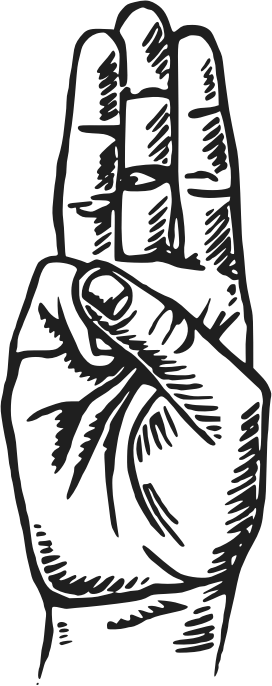
\includegraphics[scale=0.45]{img/следопытские.png}
\end{figure}
\newpage

\addcontentsline{toc}{subsection}{Будь готов}%В оглавление
\subsection*{Будь готов}
    \Am{Нас} немного пока, но мечтаем мы \F{все} об одном:\\
    \Dm{Эт}от мир изменить, озаряя душ\C{евным} огн\G{ём}.\\
    \Am{Ис}кру мысли вдохнуть в сочетании ст\F{аре}ньких слов,\\
    \Dm{Чтобы} снова гремел над страной наш дев\C{из} ``Будь гот\G{ов}!''\\
    \\    
    \-\hspace{10mm}\textbf{Припев:}\\
    \-\hspace{10mm}\Dm{Будь} готов с нами вм\G{есте} идти до конц\C{а}, \\
    \-\hspace{10mm}Будь готов удер\Am{жаться} под градом свин\Dm{ца},\\
    \-\hspace{10mm}Будь готов стать стор\G{онник}ом лучших ид\C{ей},\\
    \-\hspace{10mm}Будь готов воспи\CHORD{E7}{тать} настоящих лю\Am{дей}.\\
    \\
    По ухабам истории путь где-то -- вверх, где-то -- вниз.\\
    Как народная мудрость гласит: ``На ошибках учись!''\\
    Нелегко нам сегодня добиться реальных побед,\\
    Но гораздо трудней в одиночку бороться тебе.\\
    \\
    \-\hspace{10mm}\textbf{Припев}\\
    \\
    Мы не ``Ласковый май'', мы, скорее, суровый февраль! \\
    Шутки в сторону, видите -- здесь закаляется сталь!   \\
    Через тернии -- к звёздам, нелёгким, но верным путём, \\        
    Только за руки взявшись, мы к цели заветной придём!\\
    \\
    \-\hspace{10mm}\textbf{Припев}\\
\newpage
\addcontentsline{toc}{subsection}{Город Мастеров - Фокстрот}    %В оглавление
\subsection*{Город Мастеров}
    \begin {tabline}{1}{}{}{E,A,D,G,H,E}
        \note {1}{16}{5}{0} % we use \note instead of \notel and omit the last argument
        \note {2}{16}{5}{2}
        \note {3}{16}{5}{4}
        \note {4}{16}{4}{0}
    \end {tabline}
    \D{Если} ты устал в этой с\A{уете} дождливого дн\D{я},\\
    \G{От} скуки сходишь с ум\A{а} и на стенку зал\D{езть} готов.\\
    \D{Есть} один город, где всегд\A{а} ждут те\Hm{}{бя}!\\
    И зов\G{ётся} этот город\A{} ``Город Масте\Hm{ров}''.\\
    \\
    \-\hspace{10mm}\textbf{Припев:}\\
    \-\hspace{10mm}\Hm{Там} на верш\Fs{ине} хол\Hm{ма}, средь лесов,\\
    \-\hspace{10mm}\Hm{Зво}нкий слышится см\Fs{ех} сквозь год\G{а}.\\
    \-\hspace{10mm}\D{На} перекрёстк\A{е} розы ветр\Hm{ов}\\
    \-\hspace{10mm}Этот г\G{ород} \CHORD{F\musSharp/A}{будет} стоять всег\Hm{да}. (2 раза)\\
    \\
    В нём нет ни печали, ни горя, нет зла, нет границ.\\
    И хоть будешь искать днём с огнём -- не найдёшь в нём врагов.\\
    Здесь крепкой и верной дружбы правит закон,\\
    В этом городе ``Городе Мастеров''.\\
    \\
    \-\hspace{10mm}\textbf{Припев}\\
\newpage
\addcontentsline{toc}{subsection}{Земной простор}%В оглавление
\subsection*{Земной простор}
    Мы пройд\Am{ём} сквозь земной простор\\
    По равн\Dm{инам} и перев\E{а}лам,  \\
    По верш\Am{инам} огромных гор \\
    Сквозь земн\Dm{ой} простор небыв\G{алый}.
    \begin{gather*}
    \-\hspace{10mm}\textbf{Припев:}\\
    \-\hspace{10mm}\textup{Ведь нед\C{аром} вста\G{ёт} за\Am{ря,}}\\
    \-\hspace{10mm}\textup{Небосв\C{од} от зар\G{и} весь кр\Am{асный}.} \\
    \begin{musRepeat}
    \-\hspace{10mm}\textup{Только зн\Dm{ать} бы, что вс\E{ё} не з\Am{ря},}\\
    \-\hspace{10mm}\textup{Только зн\Dm{ать} бы, что не напр\Am{асно}.}\\
    \end{musRepeat}
    \end{gather*}\\
    Не бывает на свете чудес.\\
    Всё мы сделаем своими руками.\\
    Города, что растут до небес, \\
    Никогда не построятся сами. \\

    \-\hspace{10mm}\textbf{Припев}\\
    
    Мы пройдём сквозь земной простор.\\
    Будет много нас, и будем мы вместе.\\
    Ну а те, кто придёт потом, \\
    Пусть подхватят вот эту песню.\\

    \-\hspace{10mm}\textbf{Припев}\\ 
\newpage
\addcontentsline{toc}{subsection}{Утро в росе - Владимир Васильев}%В оглавление
\subsection*{Утро в росе}
    \vspace{-5mm}
    \begin{gather*}
    \textup{\Em{Утро} в рос\C{е}, д\D{ень} зов\Em{ёт},}\\
    \textup{\G{Солнце} в глаз\D{ищах} \C{у} реб\CHORD{H7}{ят}.}\\
    \begin{musRepeat}
    \textup{\G{Мы} восход на г\D{алстуки} б\C{ережно} кро\G{им},}  \\
    \textup{\Am{Ставь} ряды плотн\Em{ее}, н\CHORD{H7}{аш} отр\Em{яд}.}\\
    \end{musRepeat}\\
    \\
    \-\hspace{3mm}\textup{Синими ночами будит нас тревога,}\\
    \-\hspace{3mm}\textup{Эй, вставайте рядом кто не спит.}\\
    \begin{musRepeat}
    \-\hspace{3mm}\textup{Рокот барабанов гулким эхом бродит,}  \\
    \-\hspace{3mm}\textup{Галстук алым пламенем горит.}\\
    \end{musRepeat}\\
    \\
    \textup{Мы костры раздуем -- буря не погасит,}\\
    \textup{Солнцу не дадим покрыться льдом.}\\
    \begin{musRepeat}
    \textup{Мы за всё в ответе, взрослые и дети,}  \\
    \textup{На своей планете каждым днём.}\\
    \end{musRepeat}\\
    \end{gather*}
\newpage
\addcontentsline{toc}{subsection}{Город Мастеров - Илья Шульман, Владимир Васильев}%В оглавление
\subsection*{Город Мастеров}
    \Am{На} заре клубит туман,\Dm{} утренние россы.\\
    \G{}Непогоде вопреки,\C{} не боясь ветров,\\
    \F{}Беспокойный, озорной \Hm{}и многоголосый\\
    \E{}Флаг взывает в поднебесье -- \Am{}Город Мастеров. (2 раза)\\
    \\
    \-\hspace{3mm}Мы придумали его: улицы и башни,\\
    \-\hspace{3mm}Камни, гулки площадей, сумерки дворов.\\
    \-\hspace{3mm}Здесь над крышами встаёт утром барабанщик,\\
    \-\hspace{3mm}Крепко палочки сжимая, он играет дробь. (2 раза)\\

    В нём не гаснут никогда краски ярких радуг,\\
    Добрый глаз надёжных рук -- в нём не перечесть.\\
    И над городом летит конь мечты крылатый,\\
    И звучит девиз: ``Отвага, верность, труд и честь''. (2 раза)\\
    \\
    \-\hspace{3mm}Только верные друзья будут с нами рядом,\\
    \-\hspace{3mm}Только вместе сохраним мужество и честь.\\
    \-\hspace{3mm}И тогда огонь костра станет нашим флагом,\\
    \-\hspace{3mm}Полетит над городом радостная весть. (2 раза)\\
    \-\hspace{3mm}Что…\\
    \\
    На заре клубит туман, утренние россы.\\
    Непогоде вопреки, не боясь ветров,\\
    Беспокойный, озорной и многоголосый\\
    Флаг взывает в поднебесье -- Город Мастеров. (2 раза)\\

\newpage
\addcontentsline{toc}{section}{Лирика}%В оглавление
\section*{\centerline{Лирика}}
\vspace{10mm}
\begin{figure}[h]
    \centering
        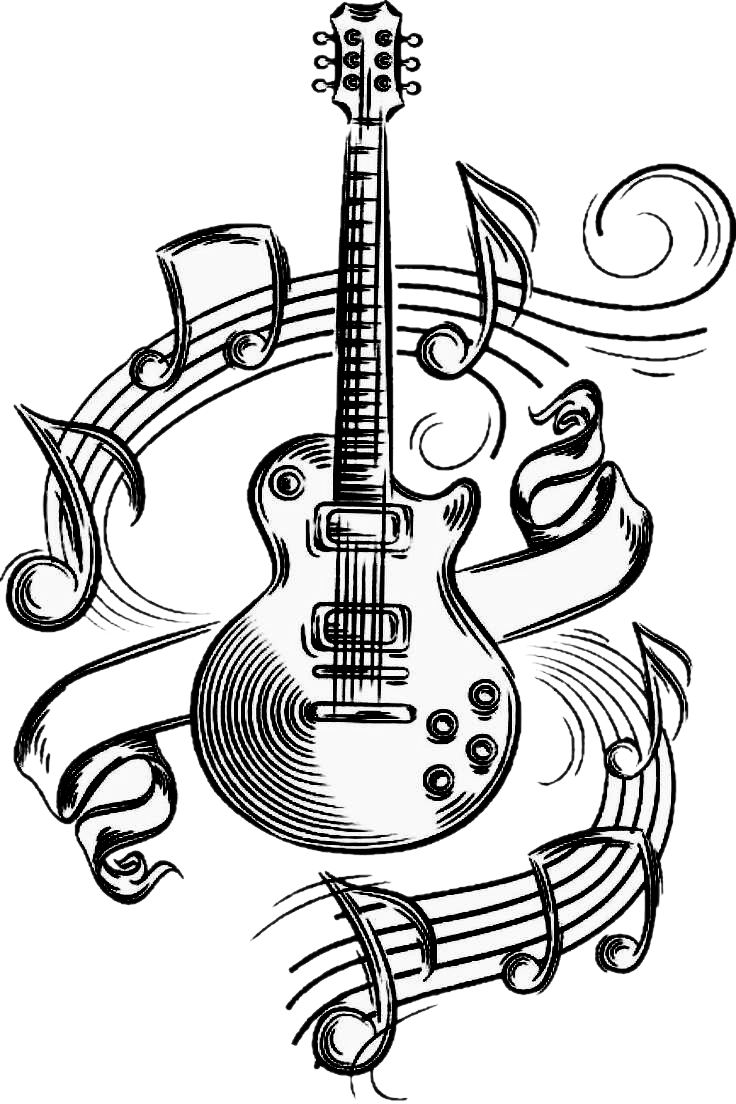
\includegraphics[scale=0.28]{img/лирика.png}
\end{figure}
\newpage
\addcontentsline{toc}{subsection}{Мой рок-н-ролл - Би-2}%В оглавление
\subsection*{Мой рок-н-ролл}
\begin {tabline}{4}{}{}{E,A,D,G,H,E}
\note{1}{8}{4}{3}
\note{2}{8}{3}{5}
\note{3}{8}{2}{0}
\note{4}{8}{3}{5}
\note{5}{8}{1}{0}
\note{6}{8}{3}{5}
\note{7}{8}{2}{0}
\note{8}{8}{3}{5}
\nextbar
\note{1}{8}{6}{3}
\note{2}{8}{3}{5}
\note{3}{8}{2}{0}
\note{4}{8}{3}{5}
\note{5}{8}{1}{0}
\note{6}{8}{3}{5}
\note{7}{8}{2}{0}
\note{8}{8}{3}{5}
\nextbar
\note{1}{8}{5}{0}
\note{2}{8}{3}{5}
\note{3}{8}{2}{0}
\note{4}{8}{3}{5}
\note{5}{8}{1}{0}
\note{6}{8}{3}{5}
\note{7}{8}{2}{0}
\note{8}{8}{3}{5}
\nextbar
\note{1}{8}{5}{0}
\note{2}{8}{3}{5}
\note{3}{8}{2}{0}
\note{4}{8}{3}{5}
\note{5}{8}{1}{0}
\note{6}{8}{3}{5}
\note{7}{8}{2}{0}
\note{8}{8}{3}{5}
\nextbar
\end {tabline}
    И \F{то}, что было, \G{набело} отк\Am{роется} потом.\\
    Мой Rock'n'Roll -- это не цель, и даже не средство,\\
    Не новое, а заново, один и об одном.\\
    Дорога -- мой дом, и для любви это не место.\\
    
    \-\hspace{10mm}\textbf{Припев:}\\
    \-\hspace{10mm}Проль\F{ются} все слова как д\G{ождь},   \\
    \-\hspace{10mm}И \Am{там}, где ты меня не ждёшь,   \\
    \-\hspace{10mm}Ночн\F{ые} ветры принес\G{ут} тебе прохла\CHORD{Am G}{ду}. \\
    \-\hspace{10mm}На наших лицах без ответа    \\
    \-\hspace{10mm}Лишь только отблески рассвета того,   \\
    \-\hspace{10mm}Где ты меня не ждёшь\\
    
    А дальше -- это главное -- похоже на тебя     \\
    В долгом пути я заплету волосы лентой,     \\
    И, не способный на покой, я знак подам тебе рукой,     \\
    Прощаясь с тобой, как будто с легендой.\\

    \-\hspace{10mm}\textbf{Припев}\\
        
    И то, что было, набело откроется потом.\\
    Мой Rock'n'Roll -- это не цель, и даже не средство,\\
    Не новое, а заново, один и об одном.\\
    Дорога -- мой дом, и для любви это не место.\\
\newpage
\addcontentsline{toc}{subsection}{Костёр - Машина Времени}%В оглавление
\subsection*{Костёр}
    \Em{Всё} отболит, и мудрый говорит: \\
    К\G{аждый} костёр \D{когда}-то догорит, \\
    В\C{етер} золу\Hm{ }развеет без сле\Em{да}.\\
    Но до тех пор, пока огонь горит, \\
    Каждый его по-своему хранит, \\
    Если беда и если холода.\\
    
    Раз ночь длинна, жгут едва-едва\\
    И берегут силы и дрова, \\
    Зря не шумят и не портят лес. \\
    Но иногда найдётся вдруг чудак,\\ 
    Этот чудак всё сделает не так. \\
    И его костёр взовьётся до небес.\\
    
    \-\hspace{10mm}\textbf{Припев}\\
    \-\hspace{10mm}\C{Ещё} не вс\G{ё} дорешен\D{о}, \C{  }ещё не в\Hm{сё} разреше\Em{но},\\
    \-\hspace{10mm}\C{Ещё} не \G{все} \A{погасли} краски дня,    \\
    \-\hspace{10mm}\C{Ещё} не жаль огня-а,\Hm{ и} Бог хранит ме\Em{ня}. \\
    
    Тот был умней, кто свой огонь сберёг, \\
    Он обогреть других уже не мог, \\
    Но без потерь дожил до тёплых дней. \\
    А ты был не прав, ты всё спалил за час, \\
    И через час большой огонь угас, \\
    Но в этот час стало всем теплей.\\
    
    \-\hspace{10mm}\textbf{Припев}\\
\newpage
\addcontentsline{toc}{subsection}{Моё сердце - Сплин}%В оглавление
\subsection*{Моё сердце}
    \vspace{-4mm}
    Мы не зн\D{али} друг друга до \G{этого} л\D{ета}\\
    Мы болт\G{ались} по св\D{ету}, земл\A{е} и во\Hm{де},\\
    И соверш\D{енно} случайно мы вз\G{яли} бил\D{еты}\\
    На сос\G{едние} кр\D{есла} на больш\A{ой} высот\Hm{е}.\musVspace\\
    \-\hspace{10mm}\textbf{Припев:}\vspace{-2mm}\\
    \-\hspace{10mm}И моё с\E{ердце} \G{о}станов\D{илось},\\
    \-\hspace{10mm}Моё с\D{ердце} з\A{ам}ерл\Hm{о},\\
    \-\hspace{10mm}И моё с\D{ердце} \G{о}станов\D{илось},\\
    \-\hspace{10mm}Моё с\D{е}рдце з\A{а}мер\Hm{ло}.\musVspace\\
    И ровно тысячу лет мы просыпаемся вместе\\
    Даже если уснули в разных местах.  \\
    Мы идём ставить кофе под Элвиса Пресли,\\
    Кофе сбежал под Propeller Heads, ах!\\
    \-\hspace{10mm}\textbf{Припев}\\
    И, может быть, ты не стала звездой в Голливуде,\\
    Не выходишь на подиум в нижнем белье.\\
    У тебя не берут автографы люди,\\
    И поёшь ты чуть тише, чем Монсерат Кабалье.\\
    Но так и я, слава богу, не Ricky, не Martin,\\
    Не выдвигался на Оскар, французам не забивал.\\
    Моим именем не назван город на карте,\\
    Но задёрнуты шторы и разложен диван.\\
    \-\hspace{10mm}\textbf{Припев}\\
    Я наяву вижу то, что многим даже не снилось,\\
    Не являлось под кайфом, не стучалось в стекло.\\
    Моё сердце остановилось, отдышалось немного\\
    И снова пошло.
\newpage
\addcontentsline{toc}{subsection}{Конь - Любэ}%В оглавление
\subsection*{Конь}
\vspace{-5mm}
    \begin{gather*}
    \textup{\Am{Выйду} ночью в п\F{оле} с кон\E{ём},}\\
    \textup{\Am{Ночкой} тёмной т\C{ихо} пойд\E{ём}.}\\
    \begin{musRepeat}
    \textup{Мы пой\Dm{дём} с кон\G{ём} п\C{о} полю вдво\F{ём}, }\\
    \textup{Мы пой\Dm{дём} с конём по п\E{олю} вдво\Am{ём}. }\\
    \end{musRepeat}\\
    \\
    \-\hspace{3mm}\textup{Ночью в поле звёзд благодать...}\\
    \-\hspace{3mm}\textup{В поле никого не видать.}\\    
    \begin{musRepeat}
    \-\hspace{3mm}\textup{Только мы с конём по полю идём,}\\      
    \-\hspace{3mm}\textup{Только мы с конём по полю идём.}\\ 
    \end{musRepeat}\\
    \\
    \textup{Сяду я верхом на коня,}\\
    \textup{Ты неси по полю меня, }\\   
    \begin{musRepeat}
    \textup{По бескрайнему полю моему, }\\     
    \textup{По бескрайнему полю моему. }\\
    \end{musRepeat}\\
    \\
    \-\hspace{3mm}\textup{Дай-ка, я разок посмотрю,}\\
    \-\hspace{3mm}\textup{Где рождает поле зарю.   }\\  
    \begin{musRepeat}
    \-\hspace{3mm}\textup{Ай, брусничный цвет, алый да рассвет, }\\     
    \-\hspace{3mm}\textup{Али есть то место, али его нет.}\\ 
    \end{musRepeat}\\
    \\
    \textup{Полюшко моё, родники,}\\
    \textup{Дальних деревень огоньки,  }\\ 
    \begin{musRepeat}
    \textup{Ой, златая рожь да кудрявый лён --}\\       
    \textup{Я влюблён в тебя, Россия, влюблён. }\\
    \end{musRepeat}\\
    \\
    \-\hspace{3mm}\textup{Будет добрым год -- хлебород,}\\
    \-\hspace{3mm}\textup{Было всяко, всяко пройдёт. }\\    
    \begin{musRepeat}
    \-\hspace{3mm}\textup{Пой, златая рожь, пой, кудрявый лён, }\\     
    \-\hspace{3mm}\textup{Пой о том, как я в Россию влюблён.}\\
    \end{musRepeat}
    \end{gather*}
\newpage
\addcontentsline{toc}{subsection}{Охота на лисицу - Green Apelsin}%В оглавление
\subsection*{Охота на лисицу}
    \Am{Да}ле-дале\Dm{ко}, в той стран\C{е}, где восходит с\E{о}лнце\\
    \Am{Ра}нним \Dm{утром} милый б\C{ольше} не просн\E{ётся}\\
    Ль\Am{ё}тся \Dm{алая} рек\C{а}, лиса сме\E{ётся}\\
    \Am{С} восточным в\Dm{етром} пусть сказ\C{ание} нес\E{ётся}\\
    \\
    В забытом ныне городе жила девица\\
    Великим самураям от любви не спится\\
    Лица жадные горят. Как не влюбиться?\\
    Но в хитрых девичьих глазах кошмар таится\\
    \\
    \-\hspace{10mm}\F{Не} беги за \Dm{нею}, глупый\\
    \-\hspace{10mm}\Am{По} её след\E{ам} идут лишь тр\F{упы}\\
    \-\hspace{10mm}В зубы кр\Dm{епче}, чем мет\E{алл}...\\
    \-\hspace{10mm}Ты по\CHORD{Am Dm C E  Am Dm C E}{пал!}\\
    \\
    По улице шагает, бедрами качая\\
    Дурак влюблённый пригласит на кружку чая\\
    Злая вслед кричит жена, свой брак спасая\\
    В нём голос совести сожрёт любовь глухая\\
    \newpage
    Под нежным платьем хвостов девять у лисицы\\
    Сведут с ума, дорожкой в гроб ведут ресницы\\
    Жрицей страсти названа, лишь единицы\\
    Оставшись в разуме, не могут с ней смириться\\
    \\
    \-\hspace{10mm}Слышен вдалеке собачий вой\\
    \-\hspace{10mm}Охота за лисьей головой\\
    \-\hspace{10mm}Сверкает в темноте оскал\\
    \-\hspace{10mm}Он попал!\\
    \\
    \F{И} в норе, где \Dm{не} достанут пс\Am{ы}\\
    Тихий шёпот р\E{аненой} лис\F{ы}\\
    Проклинает \Dm{та} свою люб\E{овь}:\\
    \\
    \Am{Яркий} мой св\Dm{ет}, скажи л\C{юбишь} или н\E{ет}\\
    Я тоб\Am{ой} была пья\Dm{на}, но дома жд\C{ёт} тебя он\E{а}\\
    Мою \Am{тайну} всем откр\Dm{ыл}, гнев мой т\C{ебя} погуб\E{ил}\\
    Местью \Am{жить} мне до кон\Dm{ца}, полюб\C{ила} я лжец\CHORD{E Am}{а...}\\
\newpage
\addcontentsline{toc}{subsection}{Что такое осень - ДДТ}%В оглавление
\subsection*{Что такое осень}
    \Am{Что} такое \E{осень} -- это \Am{небо},  \\
    \CHORD{A7}{Плачущее} небо под но\Dm{гами}.  \\
    \Dm{В} лужах разлет\E{аются} п\Am{тицы} с облак\F{ами},\\
    \Dm{Осень}, я давн\E{о} с тобою \Am{не} был\CHORD{A7}{.}\\
    \Dm{В} лужах разлет\E{аются} п\Am{тицы} с облак\F{ами},\\
    \Dm{Осень}, я давн\E{о} с тобою \Am{не} был\E{.}\\
    \\
    \-\hspace{10mm}\textbf{Припев:}\\
    \\
    \-\hspace{10mm}\Am{Осень}, в \F{небе} ж\Dm{гут} корабл\E{и}.\\
    \-\hspace{10mm}\Am{Осень}, мн\F{е} бы п\Dm{рочь} от земл\E{и}.\\   
    \-\hspace{10mm}\Dm{Там}, где в м\E{оре} \Am{тонет} печ\F{аль},\\
    \-\hspace{10mm}\Dm{Осень} -- тёмная д\E{аль}.\\
    \\
\newpage
    Что такое осень -- это камни,\\
    Верность над чернеющей Невою.\\
    Осень вновь напомнила душе о самом главном,\\
    Осень, я опять лишён покоя.\\
    Осень вновь напомнила душе о самом главном,\\
    Осень, я опять лишён покоя.  \\
    \\
    \-\hspace{10mm}\textbf{Припев}\\
    \\
    Что такое осень -- это ветер\\
    Вновь играет рваными цепями.\\
    Осень, доползём ли, долетим ли до ответа:\\
    Что же будет с родиной и с нами?\\
    Осень, доползём ли, долетим ли до рассвета?\\
    Осень, что же будет завтра с нами?\\
    \\
    \-\hspace{10mm}\textbf{Припев}\\
    \\
    Тает стаей город во мгле,\\
    Осень, что я знал о тебе?\\
    Сколько будет рваться листва?\\ 
    Осень вечно права!\begin{spacing}{0.5}
    \end{spacing}
\newpage
\addcontentsline{toc}{subsection}{Этот город - Браво}%В оглавление
\subsection*{Этот город}
    \Am{Этот} город самый лучший г\C{ород} на Зем\E{ле},\\
    \Am{Он} как будто нарисован м\F{елом} на сте\E{не}.\\
    \Dm{Нарисованы} бульвары, р\C{еки} и мосты,\\
    \Am{Разноцветные} веснушки, б\F{елые} бант\E{ы}.\\
    
    Этот город, просыпаясь, смотрит в облака,\\
    Где-то там совсем недавно пряталась луна,\\
    А теперь взрывают птицы крыльями восход,\\
    И куда-то уплывает белый пароход.\\
    
    Этот город не похожий ни на что вокруг,\\
    Улыбается прохожий и за 5 минут,\\
    Помогая человеку верить в чудеса,\\
    Распускаются фонтаны прямо в небеса.\\
    
    \-\hspace{10mm}\textbf{ Припев:}\\
    \-\hspace{10mm}\Dm{Я} не зн\CHORD{A\musSharp}{аю}, где ещ\C{ё} на \A{этом} свете \Dm{есть} так\CHORD{A\musSharp}{ая} же весн\CHORD{C A}{а}.\\  
    \-\hspace{10mm}\Dm{Я}, по\CHORD{A\musSharp}{жалуй}, отпущ\C{у} поп\A{утный} ветер \Dm{и} ос\CHORD{A\musSharp}{танусь} навсегд\C{а}... \\
    \-\hspace{10mm}(с тоб\E{ою})\\
    
    Голубые тротуары, синие цветы,\\
    Ярко-жёлтые трамваи, розовые сны.\\
    Он как будто нарисован мелом на стене,\\
    Этот город, самый лучший город на Земле  \\
    
    \-\hspace{10mm}\textbf{ Припев (2 раза)}
\newpage
\addcontentsline{toc}{subsection}{Как жаль - Браво}%В оглавление
\subsection*{Как жаль} 
    На т\G{ёмный} ряд до\Em{мов}\C{ } \\
    Лишь один\D{окий} свет в окн\CHORD{G Em C D}{е}.\\
    И стук моих шагов \\
    Звучит в полночной тишине.\\
	По этой мостовой, \\
    Вдоль этих скверов до утра,\\
	Бродили мы с тобой, \\
    И это было как вчера.\\
    
	\-\hspace{10mm}\textbf{Припев:}\\
    \-\hspace{10mm}Как ж\G{аль}, но т\C{ы} сег\H{одня} не со м\CHORD{Em D}{ной,}\\
    \-\hspace{10mm}\C{И} только к\H{аждый} \CHORD{Em D}{раз,}\\
    \-\hspace{10mm}Когда ид\C{у} по \CHORD{H7}{этой} мосто\CHORD{Em D}{вой,}\\
    \-\hspace{10mm}\C{Я} \Cm{думаю} о н\G{ас}.\\
	
    Всё так же, как тогда, \\
    Такой же мягкий лунный свет,\\
    Блестит в реке вода, \\
    И лишь тебя со мною нет.\\
 
	\-\hspace{10mm}\textbf{Припев}

\newpage
\addcontentsline{toc}{subsection}{Ты неси меня река - Любэ}%В оглавление
\subsection*{Ты неси меня река}
\begin{spacing}{0}
\begin{tabline}{4}{}{}{E,A,D,G,H,E}
\note{1}{8}{2}{1}
\note{1}{8}{3}{2}
\note{1}{8}{4}{2}
\note{1}{8}{5}{0}
\note{2}{8}{5}{0}
\note{3}{8}{5}{2}
\note{4}{8}{5}{3}
\note{5}{8}{4}{0}
\note{6}{8}{4}{2}
\note{7}{8}{3}{0}
\nextbar
\note{1}{8}{2}{1}
\note{1}{8}{3}{2}
\note{1}{8}{4}{3}
\note{1}{8}{5}{3}
\note{1}{8}{6}{1}
\note{2}{8}{3}{2}
\note{3}{8}{2}{1}
\note{4}{8}{3}{2}
\note{5}{8}{1}{1}
\note{6}{8}{3}{2}
\note{7}{8}{2}{1}
\note{8}{8}{3}{2}
\nextbar
\note{1}{8}{2}{1}
\note{1}{8}{3}{0}
\note{1}{8}{4}{2}
\note{1}{8}{5}{3}
\note{2}{8}{3}{0}
\note{3}{8}{2}{1}
\note{4}{8}{3}{0}
\note{5}{8}{1}{0}
\note{6}{8}{3}{0}
\note{7}{8}{2}{1}
\note{8}{8}{3}{0}
\nextbar
\note{1}{8}{2}{3}
\note{1}{8}{3}{0}
\note{1}{8}{4}{0}
\note{1}{8}{5}{2}
\note{1}{8}{6}{3}
\note{2}{8}{3}{0}
\note{3}{8}{2}{3}
\note{4}{8}{3}{0}
\note{5}{8}{1}{3}
\note{6}{8}{3}{0}
\note{7}{8}{2}{3}
\note{8}{8}{3}{0}
\end{tabline}
\end{spacing}%ужимаем как можем
    \Am{Ты} неси меня, ре\CHORD{F C}{ка}, за крутые берег\G{а}, где пол\Am{я...}\\
    Где поля, мои пол\F{я}, где леса\C{...} где леса, мои лес\G{а}, ты не\Am{си}...\\
    Ты неси меня, ре\CHORD{F C}{ка,} да в родные мне мест\G{а}, где жи\Am{вёт...}\\
    Где живёт моя крас\CHORD{F E7}{а,} голубые у неё гла\Am{за}.\musVspace\\
    \musVspace
    \-\hspace{10mm}\textbf{Припев:} \begin{spacing}{0.3} \end{spacing} %я изобрёл такой мтод ужима только сейчас. выглядит сурово
    \-\hspace{10mm}К\F{ак} н\C{очка} т\E{ёмн}\Am{ая},\\
    \-\hspace{10mm}К\F{ак} р\C{ечка} б\E{ыстр}\Am{ая}.\\
    \-\hspace{10mm}Как \G{оди}\Dm{нока}\E{я} лу\Am{на} --\\
    \-\hspace{10mm}На \Dm{небе} ж\Am{дёт} мен\E{я} о\Am{на}.\musVspace\\
    За туманом -- огонёк, огонёк... как же он ещё далёк. Ой, далёк...\\
    Ты мне ветер помоги -- милой весточку шепни. Знаю, ждёт...\\
    Знаю, ждёт меня краса, голубые у неё глаза.\musVspace\\
    \musVspace
    \-\hspace{10mm}\textbf{Припев}\\
    \-\hspace{10mm}\textbf{Проигрыш:} G C G Am Em F C G C C\\
    Ты нес\G{и} меня, ре\Am{ка,} за кру\Em{тые} берег\CHORD{F C G C}{а...}\\
    Ты нес\G{и} меня, ре\Am{ка,} за кру\Em{тые} берег\CHORD{F E7}{а...}\\
    Голубые у неё гла\Am{за}\musVspace\\
    \-\hspace{10mm}\textbf{Припев}
\newpage

\addcontentsline{toc}{subsection}{Искала - Земфира}%В оглавление
\subsection*{Искала}

    \Dm{Я} иск\C{ала} теб\G{я} год\A{ами} долги\Dm{ми}\\
    Иск\C{ала} теб\G{я} двор\A{ами} тёмны\Dm{ми}\\
    В журн\C{алах}, в кин\G{о}, среди друз\A{ей}\\
    В \Dm{день}, когд\C{а} нашла,\G{ }с ум\A{а} сошла\\
    \\
    \-\hspace{10mm}\textbf{Припев:}\\
    \-\hspace{10mm}Т\F{ы} совс\A{ем} как во сн\F{е}\\
    \-\hspace{10mm}Совс\A{ем} как в альб\F{омах}\\
    \-\hspace{10mm}Где \A{я} рисов\G{ала} теб\A{я} гуашью\\
    
    Дальше были звонки ночные больше\\
    Слёзы, нервы, любовь и стрелки в Польше\\
    Дети, но не мои, и старые зазнобы\\
    Куришь каждые пять, мы устали оба\\

    \-\hspace{10mm}\textbf{Припев (2 раза)}\\

    Я искала тебя годами долгими\\
    Искала тебя дворами тёмными\\
    В журналах, в кино годами долгими\\
    Искала тебя ночами-чами-чами…\\
\newpage

\addcontentsline{toc}{subsection}{ПММЛ - Земфира}%В оглавление
\subsection*{ПММЛ}

    \Am{Море} обн\G{имет}, закопает в пес\Am{ки}\\
    Зак\G{инут} рыболовы лес\Dm{ки}\\
    Пой\Em{мают} в сети наши души\Dm{}\\
    Прост\E{и} меня, моя любовь\\
    \\
    Поздно, о чём-то думать слишком поздно\\
    Тебе, я чую, нужен воздух\\
    Лежим в такой огромной луже\\
    Прости меня, моя любовь\\
    \\
    Джинсы воды набрали и прилипли\\
    Мне кажется, мы крепко влипли\\
    Мне кажется, потухло солнце\\
    Прости меня, моя любовь\\
    \\
    Тихо, не слышно ни часов, ни чаек\\
    Послушно сердце выключаем\\
    И ты в песке, как будто в бронзе\\
    Прости меня, моя любовь\\
\newpage
\addtocontents{toc}{\protect\newpage}
\addcontentsline{toc}{section}{Песни сов}%В оглавление
\section*{\centerline{Песни сов}}
\vspace{10mm}
\begin{figure}[h]
       \centering
        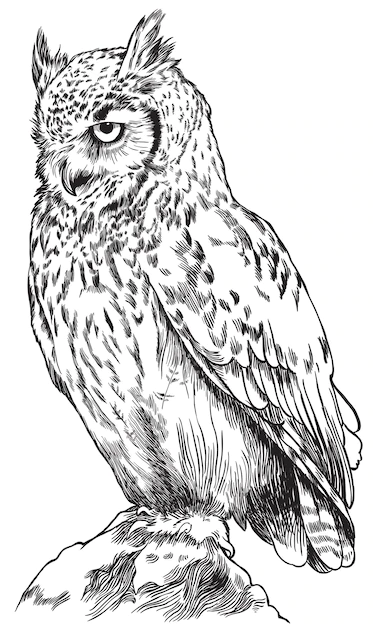
\includegraphics[scale=0.49]{img/совы.png}
\end{figure}
\newpage
\addcontentsline{toc}{subsection}{Ты, да я, да мы с тобой}%В оглавление
\subsection*{Ты, да я, да мы с тобой}
\vspace{-5mm}
    \begin{gather*}
    \textup{\Am{Ты}, да я, да мы с тобой!   Ты, да я, да мы с тобой!}\\
    \textup{\CHORD{A7}{Здорово}, когда на свете есть друзь\Dm{я}.}\\
    \begin{musRepeat}
    \textup{\Dm{Если} б жили все в один\G{очку},}\\
    \textup{Т\C{о} б уже давно на кус\F{очки} }\\
    \textup{\Dm{Развалилась} бы, на\E{верное}, Зем\CHORD{Am (A7)}{ля.}\hspace{10mm}}\\     
    \end{musRepeat}\\
    \\
    \-\hspace{3mm}\textup{Ты, да я, да мы с тобой! Ты, да я, да мы с тобой!}\\
    \-\hspace{3mm}\textup{Землю обогнём, потом махнём на Марс.  }\\
    \begin{musRepeat}
    \-\hspace{3mm}\textup{Может, у оранжевой речки   }\\
    \-\hspace{3mm}\textup{Там уже грустят человечки,  }\\
    \-\hspace{3mm}\textup{Оттого, что слишком долго нету нас.  }\\
    \end{musRepeat}\\
    \\
    \textup{Ты, да я, да мы с тобой! Ты, да я, да мы с тобой!}\\
    \textup{Нас не разлучит ничто и никогда. }\\
    \begin{musRepeat}
    \textup{Даже если мы расстаёмся,   }\\
    \textup{Дружба всё равно остаётся,   }\\
    \textup{Дружба остаётся с нами навсегда.   }\\
    \end{musRepeat}\\
    \end{gather*}
\newpage
\addcontentsline{toc}{subsection}{Город-сказка - Танцы Минус}%В оглавление
\subsection*{Город-сказка, город-мечта}
    \Dm{Я} шагаю \CHORD{A\musSharp}{по} проспекту, \Gm{по} ночному г\A{ороду}.\\
    Я иду, потому что у меня есть ноги,\\
    Я умею ходить, и поэтому иду.\\
    Иду навстречу цветным витринам,\\
    Мимо пролетают дорогие лимузины.\\
    В них женщины проносятся с горящими глазами,\\
    Холодными сердцами, золотыми волосами.\\

    \-\hspace{10mm}\textbf{Припев:}\\
    \-\hspace{10mm}\Gm{Город} -- сказка, г\A{ород} -- мечта,\\
    \-\hspace{10mm}Попа\Dm{дая} в его сети -- пропа\CHORD{A\musSharp}{даешь} навсегда.\\
    \-\hspace{10mm}Глотая воздух простуд и сквозняков,\\
    \-\hspace{10mm}С запахом бензина и дорогих духов.\\
    \-\hspace{10mm}\textbf{Проигрыш:} Gm A\\
    \\
    Звёзд на небе мало, но это не беда,\\
    Здесь почти что в каждом доме есть своя и не одна.\\
    Электричество, газ, телефон, водопровод,\\
    Коммунальный рай без хлопот и забот.\musVspace\\
    \-\hspace{10mm}\textbf{Припев}\musVspace\\
    Дым высоких труб, бег седых облаков\\
    Нам укажет приближение холодных ветров,\\
    Танец солнечных лучей в паутине проводов\\
    Над жестяными крышами обшарпанных домов.\\
    Иду навстречу цветным витринам,\\
    Мимо пролетают дорогие лимузины.\\
    В них женщины проносятся с горящими глазами,\\
    Холодными сердцами, золотыми волосами.\musVspace\\
    \-\hspace{10mm}\textbf{Припев} \\
\newpage
\addcontentsline{toc}{subsection}{Сансара - Баста}%В оглавление
\subsection*{Сансара}
    \C{Делай} вопреки, делай от руки, \\
    \Am{Мир} переверни, небо опрок\CHORD{Em (D)}{инь}. \\
    В каждом наброске, в каждом черновике, \\
    Учитель продолжается в своём ученике. \\
    Всю мою жизнь я иду ко дну,           \\ 
    Всю мою жизнь я искал любовь, чтобы любить одну. \\         
    Они сказали -- нас поздно спасать и поздно лечить.     \\    
    Плевать, ведь наши дети будут лучше, чем мы.\\
    Лучше, чем мы... Лучше, чем мы... \CHORD{Am7}{}\\

    \-\hspace{10mm}\textbf{Припев: (2 раза)}\\
    \-\hspace{10mm}\CHORD{Am7}{Когда} меня не ст\C{анет}, я буду петь голос\G{ами}\\
    \-\hspace{10mm}Мо\D{их} детей и голосами \Am{их} детей.\\
    \-\hspace{10mm}Нас просто меняют мест\C{ами},\\
    \-\hspace{10mm}Таков закон \Em{сансары}, круговор\D{от} людей. (О-о-ой, мама...) \\
    
    Нас не стереть, мы живём назло,\\
    Пусть не везёт, но мы своё возьмём. \\
    Это небо вместо сцены, здесь всё вверх ногами.\\
    И эти звёзды в темноте -- тобой зажжённый фонарик. \\
    Тысяча меня до меня, и после меня будет,\\
    Тысяча меня и в тысячах не меня, тысяча меня.\\ 
    И мы снова вдребезги и нас не починить. \\
    Плевать, ведь наши дети будут лучше, чем мы. \\
    Лучше, чем мы... Лучше, чем мы...\\

    \-\hspace{10mm}\textbf{Припев (2 раза)}
\newpage
\addcontentsline{toc}{subsection}{Дыхание - Наутилус Помпилиус}%В оглавление
\subsection*{Дыхание}
    \D{Я} просыпаюсь\A{ }в  холодном по\Hm{ту}.\\
    Я просыпаюсь\CHORD{F\musSharp}{ }в кошмарном бред\G{у}.\\
    Как будто дом наш\D{ }залило во\Em{дой},\\
    И что в живых остались \Hm{только} мы с тобой.\\
    И что над нами километры воды,\\
    И что над нами бьют хвостами киты,\\
    И кислорода не хватит на двоих.\\
    Я лежу в темноте.\\

    \-\hspace{10mm}\textbf{Припев:}\\
    \-\hspace{10mm}\Hm{Слушая} наше дых\A{ание}, я с\Hm{лушаю} наше дых\G{ание}.\\
    \-\hspace{10mm}Я \Hm{раньше} и не думал, что y н\A{ас}\\
    \-\hspace{10mm}На дво\Hm{их} с тобой одно лишь дых\G{ание}, ды\Hm{хание}.\\

     \-\hspace{10mm}\textbf{Проигрыш:} A Hm G Hm A Hm G \\
    
    Я пытаюсь разучиться дышать,\\
    Чтоб тебе хоть на минуту отдать\\
    Того газа, что не умели ценить,\\
    Но ты спишь и не знаешь,\\
    Что над нами километры воды,\\
    И что над нами бьют хвостами киты,\\
    И кислорода не хватит на двоих.\\
    Я лежу в темноте.\\
    
    \-\hspace{10mm}\textbf{Припев}    
\newpage
\addcontentsline{toc}{subsection}{Звезда по имени солнце - Виктор Цой}%В оглавление
\subsection*{Звезда по имени солнце}
    Белый с\Am{нег}, серый лёд,    \\    
    На растр\C{ескавшейся} земле.   \\
    Оде\Dm{ялом} лоскутным на ней -- \\
    Г\G{ород} в дорожной петле.   \\ 
    А над городом плывут облака,     \\   
    Закрывая небесный свет.   \\
    А над городом -- желтый дым, \\
    Городу две тысячи лет, \\
    П\Dm{рожитых} под светом Звезды по имени \Am{Солнце}...   \\ 
    \\
    \-\hspace{3mm}И две тысячи лет -- война,  \\
    \-\hspace{3mm}Война без особых причин. \\
    \-\hspace{3mm}Война -- дело молодых,\\
    \-\hspace{3mm}Лекарство против морщин. \\
    \-\hspace{3mm}Красная, красная кровь -- \\
    \-\hspace{3mm}Через час уже просто земля, \\
    \-\hspace{3mm}Через два на ней цветы и трава, \\
    \-\hspace{3mm}Через три она снова жива \\
    \-\hspace{3mm}И согрета лучами Звезды по имени Солнце... \\
    
    И мы знаем, что так было всегда,    \\
    Что судьбою больше любим,\\
    Кто живёт по законам другим \\
    И кому умирать молодым.   \\
    Он не знает слово ``да'' и слово ``нет'',\\     
    Он не помнит ни чинов, ни имён.  \\
    И способен дотянуться до звёзд, \\
    Не считая, что это сон, \\
    И упасть, опалённым Звездой по имени Солнце.\\
\newpage
\addcontentsline{toc}{subsection}{Кукушка - Виктор Цой}%В оглавление
\subsection*{Кукушка}
    \Am{Песен}, ещё не написанных, ск\C{олько}?\\
    Скажи, кук\G{ушка}\Dm{,} про\Am{пой}.\\
    В \Am{городе} мне жить или на выселках? К\C{амнем} лежать\\
    Или гореть звезд\CHORD{G Dm}{ой}? Звез\Am{дой}.\\
    
    \-\hspace{10mm}\textbf{Припев:}\\    
    \-\hspace{10mm}\G{Солнце} мо\F{ё}, взгляни на ме\Am{ня}:\\
    \-\hspace{10mm}\G{Моя} лад\F{онь} превратилась в ку\Am{лак}.\\
    \-\hspace{10mm}\G{И} если есть п\F{орох} -- дай ог\CHORD{Am G F}{ня}.\\
    \-\hspace{10mm}Вот \Am{так}.\\
    
    Кто пойдёт по следу одинокому?\\
    Сильные да смелые головы сложили в поле... В бою.\\
    Мало кто остался в светлой памяти,\\ 
    В трезвом уме да с твёрдой рукой в строю... В строю.\\
    
    \-\hspace{10mm}\textbf{Припев}\\
    
    Где же ты теперь, воля вольная,\\
    С кем же ты сейчас ласковый рассвет встречаешь? Ответь!\\
    Хорошо с тобой, да плохо без тебя.\\
    Голову да плечи терпеливые под плеть... Под плеть.\\
    
    \-\hspace{10mm}\textbf{Припев}
\newpage
\addcontentsline{toc}{subsection}{Группа крови - Виктор Цой}%В оглавление
\subsection*{Группа крови}
    \Am{Тёплое} место, но улицы ждут\\
    Отпе\Em{чатков} наших ног. \\
    \Am{Звёздная} пыль \G{-- }на сапогах.  \\
    \Am{Мягкое} кресло, клетчатый плед, \\
    Не на\Em{жатый} вовремя курок. \\
    \Am{Солнечный} день -- в ослеп\G{ительных} снах.  \musVspace\\
    \-\hspace{10mm}\textbf{Припев:}\\    
    \-\hspace{10mm}Группа к\Am{рови} -- на рукаве,\\
    \-\hspace{10mm}Мой порядковый \Em{номер} -- на рукаве,\\
    \-\hspace{10mm}Поже\Dm{лай} мне удачи в бою, пожел\G{ай} мне:\\
    \-\hspace{10mm}Не ос\Am{таться} в этой траве,\\
    \-\hspace{10mm}Не ос\Em{таться} в этой траве. \\
    \-\hspace{10mm}Поже\Dm{лай} мне удачи, пожел\G{ай} мне уд\Am{ачи}! \musVspace\\
    И есть чем платить, но я не хочу \\
    Победы любой ценой.         \\
    Я никому не хочу ставить ногу на грудь. \\
    Я хотел бы остаться с тобой, \\
    Просто остаться с тобой,\\
    Но высокая в небе звезда зовёт меня в путь. \musVspace\\
    \-\hspace{10mm}\textbf{Припев}
\newpage
\addcontentsline{toc}{subsection}{Небо славян - Алиса }%В оглавление
\subsection*{Небо славян }
    З\Em{вездопад}, да рокот зарниц. Г\Am{розы} седлают кон\G{ей}, \\
    Н\C{о} над землёй тихо л\Am{ьётся} покой м\D{о}насты\Em{рей}.  \\
    А поверх седых облаков  синь соколиная высь. \\
    Здесь, под покровом небес мы родились.\\
    \\
    След оленя лижет мороз,  гонит добычу весь день, \\
    Но стужу держит в узде дым деревень.  \\
    Намела сугробов пурга -- дочь белозубой зимы. \\
    Здесь, в окоёме снегов выросли мы.\\
    \\
    \-\hspace{10mm}\textbf{Припев:}\\
    \-\hspace{10mm}\Em{Нас} точит \Am{семя} орд\C{ы}, \Em{нас} гнет ярм\D{о} басурман, \\
    \-\hspace{10mm}\Em{Но} в наших \Am{венах} кип\C{ит} н\D{ебо} сла\Em{вян}. \\
    \-\hspace{10mm}И от Чудских берегов до ледяной Колымы. \\
    \-\hspace{10mm}Всё это наша земля! Всё это мы!\\
    \\
    За бугром куют топоры, буйные головы сечь, \\
    Но инородцам кольчугой звенит, русская речь.\\
    И от перелеска до звёзд  высится Белая рать. \\
    Здесь, на родной стороне нам помирать.\\
    \\
    \-\hspace{10mm}\textbf{Припев}
\newpage
\addcontentsline{toc}{subsection}{Однажды мир прогнётся под нас - Машина Времени}%В оглавление
\subsection*{Однажды мир прогнётся под нас}

    Вот \Em{море} молод\D{ых} колышат с\C{упер}-басы,\\
    Мне т\CHORD{H7}{риста} лет, я выполз из тьм\Em{ы}.\\
    Он\Em{и} торчат под р\D{ейв} и чем-то п\C{удрят} носы,\\
    \CHORD{H7}{Они} не такие, как \Em{мы}.  \\
    И \Am{я} не горю желаньем лезть в чужой монастырь,\\
    Я видел эту жизнь без прик\CHORD{H7}{рас}...\\
    Не с\Em{тоит} прогиб\D{аться} под изм\A{енчивый} м\C{ир},\\
    Пусть \CHORD{H7}{лучше} он прогнётся под \Em{нас},\\
    Одн\C{ажды} он прогнётся под \Em{нас}.\\
    
    \-\hspace{3mm}Один мой друг -- он стоил двух. Он ждать не привык, \\
    \-\hspace{3mm}Был каждый день последним из дней.        \\       
    \-\hspace{3mm}Он пробовал на прочность этот мир каждый миг --  \\ 
    \-\hspace{3mm}Мир оказался прочней.  \\
    \-\hspace{3mm}Ну что же, спи спокойно, позабытый кумир,       \\                 
    \-\hspace{3mm}Ты брал свои вершины не раз...     \\   
    \-\hspace{3mm}Не стоит прогибаться под изменчивый мир, \\          
    \-\hspace{3mm}Пусть лучше он прогнётся под нас,       \\
    \-\hspace{3mm}Однажды он прогнётся под нас.\\
\newpage
    Другой держался русла и теченье ловил  \\
    Подальше от крутых берегов.      \\
    Он был, как все, и плыл, как все, и вот он приплыл -- \\ 
    Ни дома, ни друзей, ни врагов.  \\
    И жизнь его похожа на фруктовый кефир,         \\             
    Видал я и такое не раз...\\
    Не стоит прогибаться под изменчивый мир,     \\      
    Пусть лучше он прогнётся под нас,    \\        
    Однажды он прогнётся под нас.\\
    
    \-\hspace{3mm}Пусть старая джинса давно затерта до дыр,     \\                      
    \-\hspace{3mm}Пускай хрипит раздолбанный бас...\\
    \-\hspace{3mm}Не стоит прогибаться под изменчивый мир,    \\      
    \-\hspace{3mm}Пусть лучше он прогнётся под нас,  \\     
    \-\hspace{3mm}Однажды он прогнётся под нас,      \\ 
    \-\hspace{3mm}Однажды он прогнётся под нас,   \\   
    \-\hspace{3mm}Однажды он прогнётся под нас.\\
\newpage
\addcontentsline{toc}{subsection}{Враг - Кошка Сашка}%В оглавление
\subsection*{Враг}
    \Am{Как} с утра набеж\F{али} тучи, \C{а} теперь светит м\E{есяц} ясный.\\
    Горько плачет краса-Маруся, только это теперь напрасно.\\
    Парень статный, хмельное лето, да под осень пришла повестка,\\
    Сколько песен об этом спето, для чего же такая песня?       \\                            
    Звёзды светят, девчонка плачет, а парнишке другое снится:\\
    Автомат, да вагон удачи, чтобы бой, чтобы ветер в лица,\\
    Чтобы он да удар пропустит не бывало ещё ни разу.\\
    Завтра встанет, да песню в зубы, \\
    Мать обнимет, да прыгнет в газик.\\
    \Dm{И} вместо прощ\E{анья} махнув из ок\Am{на} загорелой рук\F{ой,}\\
    Рванётся туда, где в дыму и слезах начинается бой,\\
    Где звёзды горят вместе с небом, от дыма не видно ни зги,\\
    Где за лесом речка, за речкою фронт, а за фронтом враги.\\
    \\
    \-\hspace{10mm}\textbf{Припев:}\\
    \-\hspace{10mm}\Dm{Враг} навсегда оста\E{ётся} врагом,\\
    \-\hspace{10mm}Не де\Am{ли} с ним хлеб, не зов\F{и} его в дом,\\
    \-\hspace{10mm}Даже \C{если} пока воздух м\E{иром} запах,\\
    \-\hspace{10mm}Он, хо\Am{тя} и спокойный, но вс\F{е}-таки враг.\\
    \-\hspace{10mm}Если \Dm{он}, как и ты, не проп\E{ил} свою честь,\\
    \-\hspace{10mm}Враг не \Am{может} быть бывшим, он б\F{удет} и есть.\\
    \-\hspace{10mm}Будь же в\C{ерен} прицел, и не др\E{огни} рука,\\
    \-\hspace{10mm}Ты по\Am{гибнешь} когда, пожалеешь враг\F{а}.
    \newpage
    Автомат, да вагон удачи, только парень опять не весел...\\
    Письма ходят, девчонка плачет, добавляя куплеты в песню.\\
    Уже год идет наступленье, и пылают чужие хаты,\\
    Враг бежит, но что интересно, что похожи вы с ним как братья.\\
    Как и ты дрался с пацанами со двора, руки разбивая,\\
    Провожали его ребята, и девчонка его, рыдая,\\
    И обидно, что случай дался б, он бы бил бы тебя с лихвою --\\
    Коль однажды врагом назвался, будь хотя бы врагом-героем.\\
    \\
    И вместо проклятий ему, посвящая живые стихи,\\
    Смеёшься о том, что не смерть бы, а водку из этой руки.\\
    Дрожит в амбразуре закат, и ухмылка ползет по щекам,\\
    Как славно бы выпить сейчас по 100 грамм таким лютым врагам, но\\
    \\
    \-\hspace{10mm}\textbf{Припев}\\
    \\
    Это присказка, а не сказка, на войне горе воет волком.\\
    Слово ``Лирика'' здесь опасно, тот, кто ноет, живет недолго.\\
    Дан приказ -- он оборонялся, в темноту по тебе стреляя.\\
    По горам ты за ним гонялся, по себе его вычисляя.\\
    Те же жесты, одни привычки, Боже, может и вправду братья.\\
    Не убить -- самому не выжить, ох прийти расспросить бы батю.\\
    А в прицеле дрожало небо, слёз не пряча и бой был долгим.\\
    Жаль, что он тебе другом не был, ты сильнее, и слава Богу.\\
    \\
    И вместо молитв к небесам посылаешь последний патрон\\
    На память о том кто был честен и смел, но назвался врагом\\
    Ну вот и закончилась песня, и в общем, закончился бой.\\
    Ну что же ты грустен приятель, теперь твоя правда с тобой\\
    
    \-\hspace{10mm}\textbf{Припев}
\newpage
\addcontentsline{toc}{subsection}{Маленький - Дайте танк (!)}%В оглавление
\subsection*{Маленький}
    \begin {tabline}{4}{}{}{E,A,D,G,H,E}
        \note{1}{8}{1}{2}
        \note{1}{8}{2}{2}
        \note{1}{8}{3}{2}
        \note{1}{8}{4}{4}
        \note{1}{8}{5}{4}
        \note{1}{8}{6}{2}
        \note{3}{8}{1}{2}
        \note{3}{8}{2}{2}
        \note{3}{8}{3}{2}
        \note{3}{8}{4}{4}
        \note{3}{8}{5}{4}
        \note{3}{8}{6}{2}
        \note{5}{8}{1}{2}
        \note{6}{8}{2}{5}
        \note{7}{8}{2}{2}
        \note{8}{8}{1}{2}
        \note{8}{8}{2}{2}
        \note{8}{8}{3}{2}
        \note{8}{8}{4}{4}
        \note{8}{8}{5}{4}
        \note{8}{8}{6}{2}
        \nextbar
        \note{1}{8}{1}{0}
        \note{1}{8}{2}{0}
        \note{1}{8}{3}{1}
        \note{1}{8}{4}{2}
        \note{1}{8}{5}{2}
        \note{1}{8}{6}{0}
        \note{3}{8}{1}{0}
        \note{3}{8}{2}{0}
        \note{3}{8}{3}{1}
        \note{3}{8}{4}{2}
        \note{3}{8}{5}{2}
        \note{3}{8}{6}{0}
        \note{5}{8}{1}{2}
        \note{6}{8}{1}{0}
        \note{7}{8}{2}{2}
        \note{8}{8}{1}{0}
        \note{8}{8}{2}{0}
        \note{8}{8}{3}{1}
        \note{8}{8}{4}{2}
        \note{8}{8}{5}{2}
        \note{8}{8}{6}{0}
        \nextbar
        \note{1}{8}{1}{2}
        \note{1}{8}{2}{2}
        \note{1}{8}{3}{2}
        \note{1}{8}{4}{4}
        \note{1}{8}{5}{4}
        \note{1}{8}{6}{2}
        \note{3}{8}{1}{2}
        \note{3}{8}{2}{2}
        \note{3}{8}{3}{2}
        \note{3}{8}{4}{4}
        \note{3}{8}{5}{4}
        \note{3}{8}{6}{2}
        \note{5}{8}{2}{2}
        \note{6}{8}{2}{5}
        \note{7}{8}{2}{2}
        \note{8}{8}{1}{2}
        \note{8}{8}{2}{2}
        \note{8}{8}{3}{2}
        \note{8}{8}{4}{4}
        \note{8}{8}{5}{4}
        \note{8}{8}{6}{2}
        \nextbar
        \note{1}{8}{1}{0}
        \note{1}{8}{2}{0}
        \note{1}{8}{3}{1}
        \note{1}{8}{4}{2}
        \note{1}{8}{5}{2}
        \note{1}{8}{6}{0}
        \note{3}{8}{1}{0}
        \note{3}{8}{2}{0}
        \note{3}{8}{3}{1}
        \note{3}{8}{4}{2}
        \note{3}{8}{5}{2}
        \note{3}{8}{6}{0}
        \note{5}{8}{1}{2}
        \note{6}{8}{1}{0}
        \note{7}{8}{2}{2}
        \note{8}{8}{1}{0}
        \note{8}{8}{2}{0}
        \note{8}{8}{3}{1}
        \note{8}{8}{4}{2}
        \note{8}{8}{5}{2}
        \note{8}{8}{6}{0}
    \end{tabline}
    Я снова \CHORD{F\musSharp{}m}{маленький}, солнце яркое,\\
    Мама оп\E{ять} сильнее всех в мире,\\
    Я с\CHORD{F\musSharp{}m}{}нова боюсь собак\\
    И остав\E{}аться один в квартире,\\
    А де\Hm{}ревья такие большие,\\
    Незнак\D{}омы плохие слова;\\
    Поиграем в п\CHORD{F\musSharp{}m}{}рятки?\\
    Мне как р\E{}аньше по пояс трава.\\
    \\
    \-\hspace{10mm}\textbf{Припев:}\\
    \-\hspace{10mm}Это \D{}я не доста\E{}ю до пола но\CHORD{F\musSharp{}m}{}гами\\
    \-\hspace{10mm}Или пол до моих ног не достаёт?\\
    \-\hspace{10mm}Те, кого я считал врагами,\\
    \-\hspace{10mm}Просто делают мёд, просто делают мёд...\\
    \-\hspace{10mm}Это я, только дети трясут головами --\\
    \-\hspace{10mm}Не узнали меня, говорят, что не смогут помочь;\\
    \-\hspace{10mm}Я стал сильнее и теперь я не лягу к маме,\\
    \-\hspace{10mm}Но чудовища не пришли -- я прождал их целую ночь.\musVspace\\
    \-\hspace{10mm}\textbf{Проигрыш:} D E\\
\newpage
    Я ещё не разучился радоваться,\\
    Рисую осколками кирпичей,\\
    В резиновых сапогах не страшно\\
    Мерить весной ногами ручей,\\
    Красные яблоки падают вниз,\\
    Когда ветер сильнее дует;\\
    Тише, меня зовут есть!\\
    Я не голоден, но никого не волнует.\\
    
    \-\hspace{10mm}\textbf{Припев}\\
  
    Снова зима, меня везут на санках,\\
    Снеговик до утра подождёт,\\
    А дома тепло и пахнет ёлкой,\\
    В клубок свернулся кот;\\
    Вот моё отражение в шаре,\\
    Гирлянда мигает цветными огнями,\\
    Я сижу на скрипучем стуле\\
    И не достаю до пола ногами.\\
    
    \-\hspace{10mm}\textbf{Припев}
\newpage
\addcontentsline{toc}{subsection}{Алые паруса - В. Ланцберг}%В оглавление
\subsection*{Алые паруса - В. Ланцберг}
\vspace{-5mm}
    \begin{gather*}
    \textup{Ре\Am{бята}, надо верить в чуде\Dm{са}!}\\
    \textup{Ког\G{да}-нибудь, весенним утром р\C{анним}},\\
    \begin{musRepeat}
    \textup{Над \Dm{океаном} \G{алые} взметн\C{утся} пару\Am{са,}}\\
    \textup{И ск\Dm{рипка} пропо\E{ёт} над оке\CHORD{Am (A)}{аном}.}   \\     
    \end{musRepeat}\\
    \\
    \-\hspace{3mm}\textup{Не три глаза, ведь это же не сон.}\\
    \-\hspace{3mm}\textup{И алый парус правды гордо реет,}\\
    \begin{musRepeat}
    \-\hspace{3mm}\textup{В той бухте, где отважный Грей нашёл свою Ассоль,}\\
    \-\hspace{3mm}\textup{В той бухте, где Ассоль дождалась Грея.}\\
    \end{musRepeat}\\
    \\
    \textup{С друзьями легче море переплыть}\\
    \textup{И съесть морскую соль, что нам досталась.}\\
    \begin{musRepeat}
    \textup{А без друзей на свете было б очень трудно жить,}\\
    \textup{И серым стал бы даже алый парус.}\\
    \end{musRepeat}\\
    \\
    \-\hspace{3mm}\textup{Ребята, надо верить в чудеса!}\\
    \-\hspace{3mm}\textup{Когда-нибудь, весенним утром ранним,}\\
    \begin{musRepeat}
    \-\hspace{3mm}\textup{Над океаном алые взметнутся паруса},\\
    \-\hspace{3mm}\textup{И скрипка пропоет над океаном.}\\
    \end{musRepeat}
    \end{gather*}
\newpage
\addcontentsline{toc}{subsection}{Луч солнца золотого - Муслим Магомаев(ст. Юрий Энтин)}%В оглавление
\subsection*{Луч солнца золотого}
    Л\C{}уч солнца золо\Em{}того ть\Am{}мы скрыла пелен\C{}а.\\
    \C{}И между нами с\Em{}нова вдр\F{}уг выросла стен\E{}а.\\
    А-а-\F{}а, а-а-\G{}а-а-а.\\ 

    \-\hspace{10mm}\textbf{Припев:}\\
    \-\hspace{10mm}\C{}Ночь пройдёт, наступит \F{}утро \G{}ясное,\\
    \-\hspace{10mm}Знаю, счастье нас с тобой ждёт. \\
    \-\hspace{10mm}Ночь пройдёт, пройдёт пора ненастная,\\
    \-\hspace{10mm}С\C{}олнце взой\CHORD{Am F G}{}дёт! (2 раза)\\

    Петь птицы перестали, свет звёзд коснулся крыш.\\
    В час грусти и печали ты голос мой услышь.\\
    А-а-а, а-а-а-а-а. \\
 
   \-\hspace{10mm}\textbf{Припев}
\newpage
\addcontentsline{toc}{subsection}{Потерянный рай - Ария}%В оглавление
\subsection*{Потерянный рай}
\vspace{-4.0mm}
    \begin{spacing}{0.9}
    \CHORD{Am7}{О}т края до края \CHORD{D7}{н}ебо в огне сгорает,\\
    \CHORD{Fmaj7}{И} в нём исчезают все над\C{ежды} и мечт\G{ы}.\\
     Но ты засыпаешь, и ангел к тебе слетает,\\
    Смахнёт твои слёзы, и во сне смеёшься ты!\musVspace\\
    \-\hspace{10mm}\textbf{Припев:}\vspace{-2mm}\\
    \-\hspace{10mm}Засып\F{ай}, на рук\G{ах} y меня засып\Am{ай},\\
    \-\hspace{10mm}Засып\F{ай} \G{под} пенье дожд\Am{я...}\\
    \-\hspace{10mm}Далек\F{о}, там, где н\G{еба} кончается к\CHORD{Am G C D}{рай},\\
    \-\hspace{10mm}Ты найд\F{ёшь} \G{потерянный} \Am{рай}.\musVspace\\
    Во сне хитрый демон может пройти сквозь стены,\\
    Дыханье y спящих он умеет похищать.\\
    Бояться не надо, душа моя будет рядом,\\
    Твои сновиденья до рассвета охранять.\musVspace\\
    \-\hspace{10mm}\textbf{Припев} \vspace{-2mm}\\
    \Hm{Подставлю} ладони -- их б\E{олью} своей наполни,\\
    \G{Наполни} печалью, страхом г\D{улкой} темнот\A{ы},\\
    И ты не узнаешь, как небо в огне сгорает,\\
    И жизнь разбивает все надежды и мечты.\musVspace\\
    \-\hspace{10mm}\textbf{Припев:}\vspace{-2mm}\\
    \-\hspace{10mm}Засып\G{ай}, на рук\A{ах} y меня засып\Hm{ай},\\
    \-\hspace{10mm}Засып\G{ай} \A{под} пенье дожд\Gm{я...}\\
    \-\hspace{10mm}Далек\G{о}, там, где н\A{еба} кончается к\CHORD{Hm A D E}{рай},\\
    \-\hspace{10mm}Ты найд\G{ёшь} \A{потерянный} \Hm{рай}.
    \end{spacing}
\newpage

\addcontentsline{toc}{subsection}{Капитал - Ляпис Трубецкой}%В оглавление
\subsection*{Капитал}
    Я \Am{ем} на об\F{ед} \Dm{золотые} сл\E{итки}\\
    Бриллиантовый десерт, нефтяные сливки\\
    Мне имя Вельзевул, хозяин стратосферы\\
    Я нереальный cool, мой респект без меры\\
    \\
    \-\hspace{10mm}\textbf{Припев :}\\  
    \-\hspace{10mm}В левой руке -- ``Snickers'', в правой руке -- ``Mars''\\
    \-\hspace{10mm}Мой пиар-менеджер -- Карл Маркс\\
    \-\hspace{10mm}В левой руке -- ``Snickers'', в правой руке -- ``Mars''\\
    \-\hspace{10mm}Мой пиар-менеджер -- Карл Маркс\\
    \-\hspace{10mm}Капитал! Капитал! Капитал! Капитал!\\
    \\
    Я ем города, морями запиваю\\
    Моя борода небо заслоняет\\
    Гром и молнии, туманы и дожди\\
    Мои ботинки лижут министры и вожди\\
    \\
    \-\hspace{10mm}\textbf{Припев}\\  
    \\
    \-\hspace{10mm}В левой руке -- ``Snickers'', в правой руке -- ``Mars''\\
    \-\hspace{10mm}Мой пиар-менеджер -- Карл Маркс\\
    \-\hspace{10mm}Моё лицо -- Мадонна, внутри из тухлых груш\\
    \-\hspace{10mm}Все на колени! Оркестр, туш!\\
    \-\hspace{10mm}Капитал! Капитал! Капитал! Капитал!\\
    \-\hspace{10mm}Капитал! Капитал! Капитал! Капитал!\\
\newpage
\addcontentsline{toc}{subsection}{Гореть - Lumen}%В оглавление
\subsection*{Гореть}
    \vspace{-3.0mm}
    \Am{Зачем} крич\G{ать}, когда никто не сл\F{ышит}, о чём мы говор\Dm{им}. \\
    \Am{Мне} кажется, что м\G{ы} давно не ж\F{ивы}, зажглись и поти\Dm{хоньку} догорим.\\
    \F{Когда} нас м\Am{ного} начинается пож\G{ар}, и города пох\F{ожи} на крематорий и базар. \\
    И все привыкли ниче\Am{го} не замечать. Когд\G{а} тебя не слышат, дл\F{я} чего кричать? \musVspace\\
    \-\hspace{10mm}\textbf{Припев:}\\
    \-\hspace{10mm}\Dm{Мы} можем помол\Am{чать}, мы можем п\C{еть},\\
    \-\hspace{10mm}Стоять или беж\G{ать}, но всё равно гор\Dm{еть}.\\
    \-\hspace{10mm}Огромный синий \Am{кит} порвать не может с\C{еть},\\
    \-\hspace{10mm}Сдаваться или н\G{ет}, но всё-равно гор\Dm{еть}. \musVspace\\
    И снова небо замыкает на себя слова и провода. \\
    И снова с неба проливаются на нас ответы и вода. \\
    И если ты вдруг начал что-то понимать, и от прозрений захотелось заорать, \\
    Давай кричи, но тебя могут не понять, никто из них не хочет ничего менять! \musVspace\\
    \musVspace
    \-\hspace{10mm}\textbf{Припев:}\\
    \-\hspace{10mm}Мы можем помолчать, мы можем петь, \\
    \-\hspace{10mm}Стоять или бежать, но всё равно гореть! \\
    \-\hspace{10mm}Гори, но не сжигай, иначе скучно жить, \\
    \-\hspace{10mm}Гори, но не сжигай. Гори, чтобы светить... \musVspace \\
    \textbf{Проигрыш:} F Am G F | Am G F\\
\newpage
\addcontentsline{toc}{section}{Песни жаворонков}%В оглавление
\section*{\centerline{Песни жаворонков}}
\vspace{10mm}
\begin{figure}[h]
       \centering
        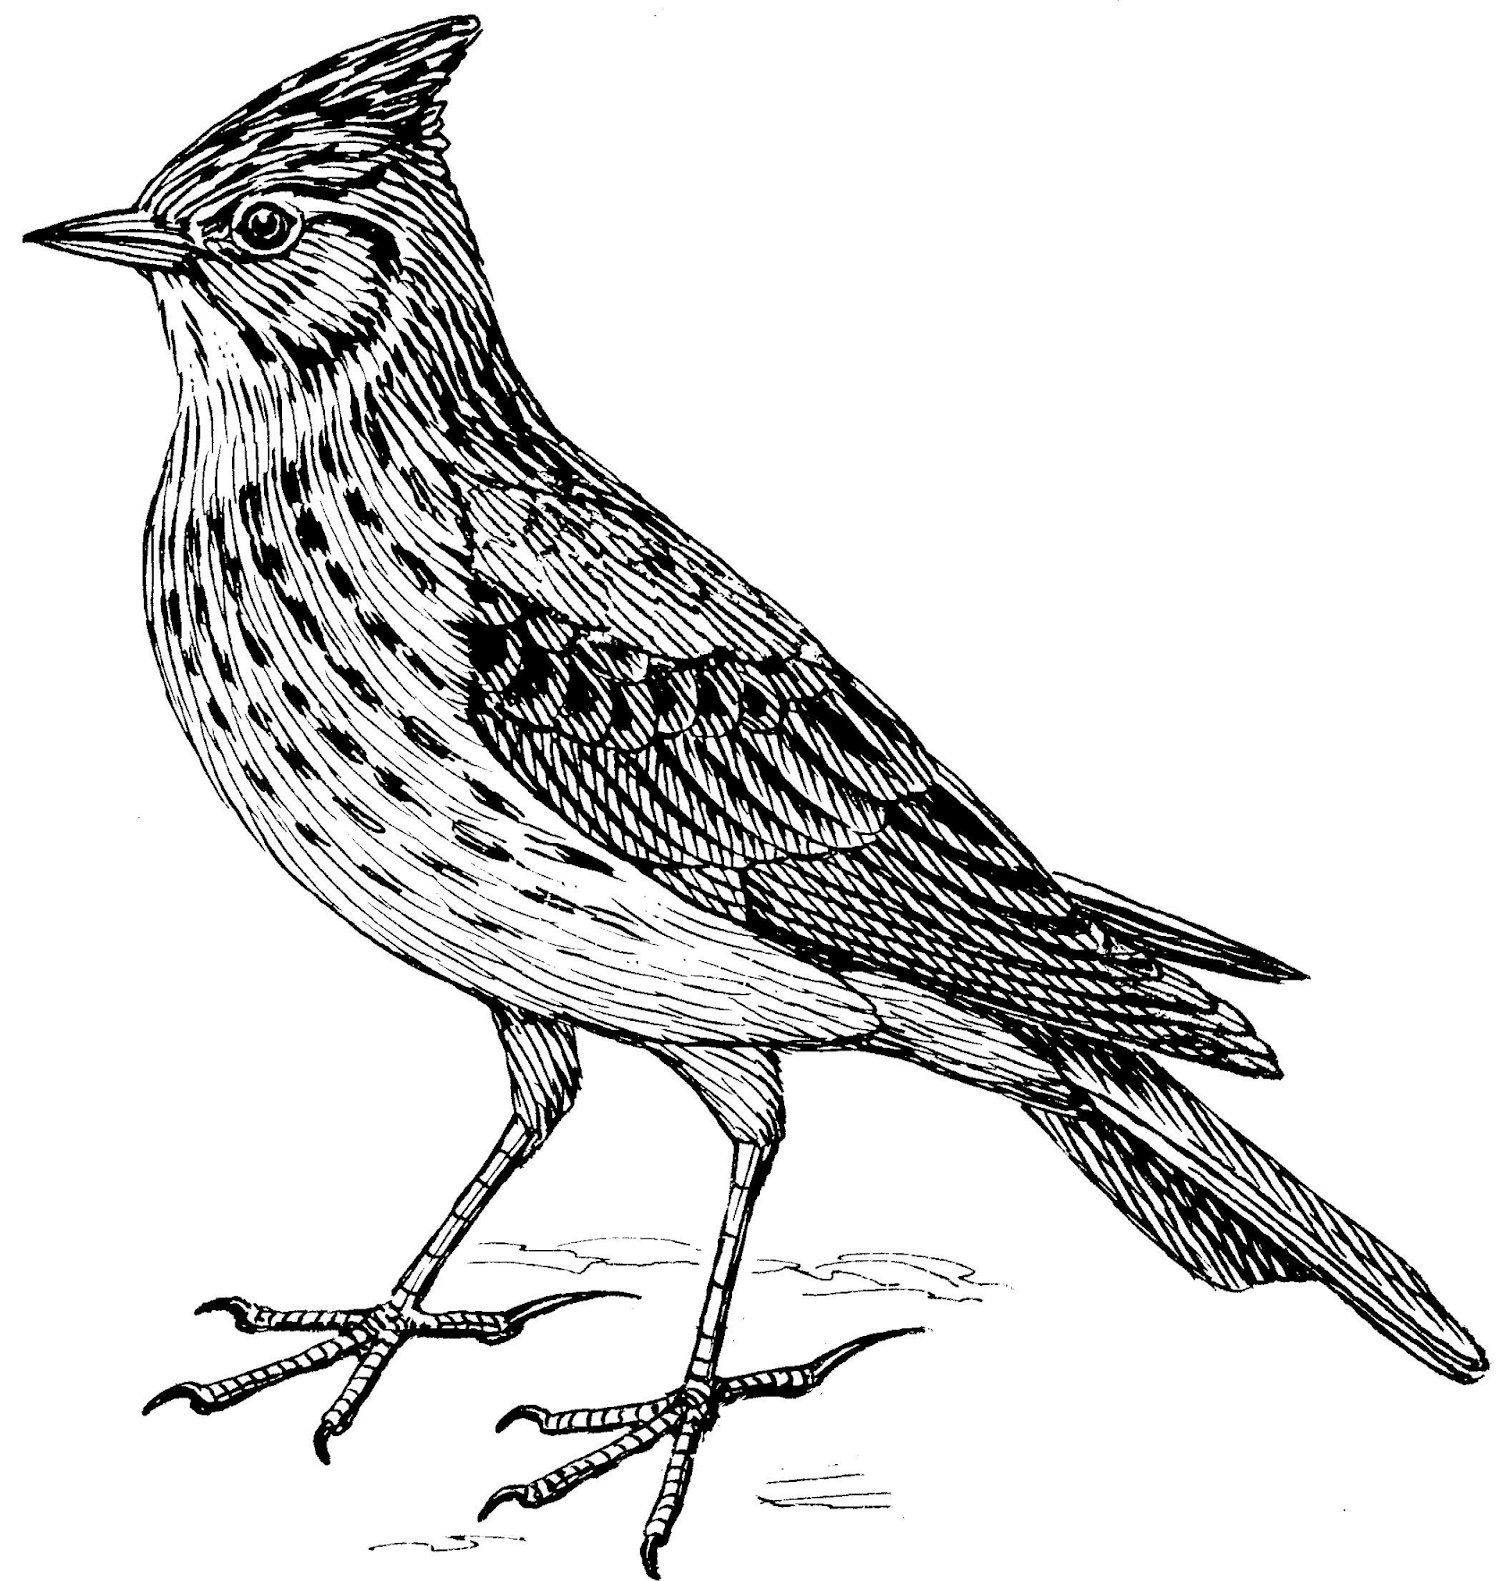
\includegraphics[scale=0.25]{img/жаворонки.png}
\end{figure}
\newpage
\addcontentsline{toc}{subsection}{Не бывает - В. Васильев (ст. М. Пляцковский)}%В оглавление
\subsection*{Не бывает}
\vspace{-3mm}
    З\Em{най}, что не бы\Am{вает} \CHORD{H7}{лодки} без ре\Em{ки},\\
    Пр\D{аздника} -- без песни, хлеба -- без мук\G{и},\\
    Д\E{ождика} -- без \Am{тучки}, р\D{озы} -- без шип\G{ов,}\\
    С\Am{казок} \CHORD{Am/C Em Em/G H7}{-- без} начала, леса -- без гри\Em{бов}.\musVspace\\
    \-\hspace{10mm}\textbf{Припев:}\\
    \-\hspace{10mm}Не бы\CHORD{Am Am/C H7}{вает}... Не бы\CHORD{Em Em/G Em Em/G}{вает}...\\
    \-\hspace{10mm}\CHORD{Am Am/C}{Дождика} -- без \CHORD{ Em Em/G H7 }{тучки}, розы -- без ши\Em{пов,}\\
    \-\hspace{10mm}Не бывает... Не бывает...\\
    \-\hspace{10mm}Сказок -- без начала, леса -- без грибов.\musVspace\\
    Знай, что не бывает моря без волны,\\
    Шутки -- без улыбки, марта -- без весны,\\
    Лётчиков -- без неба, армий -- без полков,\\
    Школ -- без переменок, драк -- без синяков.\musVspace\\
    \-\hspace{10mm}\textbf{Припев:}\\
    \-\hspace{10mm}Не бывает... Не бывает...\\
    \-\hspace{10mm}Лётчиков -- без неба, армий -- без полков,\\
    \-\hspace{10mm}Не бывает... Не бывает...\\
    \-\hspace{10mm}Школ -- без переменок, драк -- без синяков.\musVspace\\
    Знай, что не бывает дружбы без друзей,\\
    Лестниц -- без ступенек, а дома -- без дверей,\\
    Утра -- без рассвета, дыма -- без огня...\\
    В общем продолжайте дальше без меня.\musVspace\\
    \-\hspace{10mm}\textbf{Припев:}\\
    \-\hspace{10mm}Не бывает... Не бывает...\\
    \-\hspace{10mm}Утра -- без рассвета, дыма -- без огня...\\
    \-\hspace{10mm}Не бывает... Не бывает...\\
    \-\hspace{10mm}В общем продолжайте дальше без меня.\\
\newpage
\addcontentsline{toc}{subsection}{Алые паруса}%В оглавление
\subsection*{Алые паруса}
    У с\C{инего} моря, где бу\Am{шуют} бураны,\\
    Жи\Dm{ла} там девчонка с \G{именем} странным.\\
    И часто бывало: она на просторе \\
    В мечтах уплывала за синее море.\\
    
    \-\hspace{10mm}\textbf{Припев:}\\
    \-\hspace{10mm}\C{Алые} паруса. (Ассоль)     \\           
    \-\hspace{10mm}\Am{Алые} паруса. (Плюс Грей) \\             
    \-\hspace{10mm}\Dm{Алые} п\G{аруса}, парус\C{а}.\\
    
    А там за морями, за синей чертою.\\
    Жил парень отважный с открытой душою.\\
    Мечтал он о море, о странствиях дальних.\\
    Мечтал о походах в дальние страны.\\
    
    \-\hspace{10mm}\textbf{Припев}\\
    
    И вечером поздним, когда все уснули,\\
    На небе зажглись миллионы огней.\\
    И этой же ночью случилось чудо:\\
    Тот парень с девчонкой влюбились друг в друга.\\
    
    \-\hspace{10mm}\textbf{Припев}
\newpage
\addcontentsline{toc}{subsection}{Землю обмотали - Е. Птичкин (ст. М Пляцковский)}%В оглавление
\subsection*{Землю обмотали}
\vspace{-5mm}
    \begin{gather*}
    \textup{\Am{Землю} обмотали \Dm{тоненькие} нити: }\\
    \textup{\CHORD{E7}{Нити} параллелей \Am{и} зелёных рек, }\\
    \begin{musRepeat}
    \textup{\CHORD{A7}{Совершите} чудо -- \Dm{руку} протяните, }\\
    \textup{\Am{Надо}, чтобы в д\Dm{ружбу} верил \CHORD{E7}{каждый} чело\CHORD{A7}{век}. }\\
    \end{musRepeat} \\
    \\
    \-\hspace{3mm}\textup{Обогрейте словом, обласкайте взглядом,}\\
    \-\hspace{3mm}\textup{От весёлой шутки тает даже снег,}\\
    \begin{musRepeat}
    \-\hspace{3mm}\textup{Это так чудесно, если с вами рядом}\\
    \-\hspace{3mm}\textup{Улыбнётся незнакомый хмурый человек. }\\
    \end{musRepeat}\\
    \\
    \textup{Мы не зря мечтали о волшебном чуде,  }\\
    \textup{Пусть планету кружит всемогущий век,}\\
    \begin{musRepeat}
    \textup{Совершите чудо -- пусть выходит в люди, }\\
    \textup{Пусть выходит, пусть выходит в люди человек. }\\
    \end{musRepeat}\\
    \end{gather*}
\newpage
\addcontentsline{toc}{subsection}{Дорога добра - М. Минков (ст. Юрий Энтин)}%В оглавление
\subsection*{Дорога добра}
\vspace{-5mm}
    \begin{gather*}
    \textup{Спро\Dm{си} у жизни строгой, ка\Gm{кой} ид\CHORD{A7}{ти} до\Dm{рогой},} \\
    \textup{Ку\Dm{да} по свету б\F{елому} отп\CHORD{A\musSharp}{равитьс}\C{я} с утр\F{а}. }\\
    \begin{musRepeat}
    \textup{Иди за \CHORD{D7}{со}лн\Gm{цем} с\CHORD{A7}{ледом}, хоть \Dm{этот} \CHORD{Dm/C}{путь} не\CHORD{A\musSharp}{ведом}, }\\
    \textup{И\Gm{ди}, мой друг, всег\Dm{да} иди до\Gm{ро}го\CHORD{A7}{ю} доб\Dm{ра}.}\\ 
    \end{musRepeat}\\
    \\
    \-\hspace{3mm}\textup{Забудь свои заботы, падения и взлёты, }\\
    \-\hspace{3mm}\textup{Не хнычь, когда судьба себя ведёт не как сестра.} \\
    \begin{musRepeat}
    \-\hspace{3mm}\textup{Но если с другом худо, не уповай на чудо, }\\
    \-\hspace{3mm}\textup{Спеши к нему, всегда веди дорогою добра.}  \\
    \end{musRepeat}\\
    \\
    \textup{Ах, сколько будет разных сомнений и соблазнов, }\\
    \textup{Не забывай, что это жизнь, не детская игра.} \\
    \begin{musRepeat}
    \textup{Ты прочь гони соблазны, усвой закон негласный, }\\
    \textup{Иди, мой друг, всегда иди дорогою добра.}\\
    \end{musRepeat}
    \end{gather*}
\newpage
\addcontentsline{toc}{subsection}{33 коровы - М. Дунаевский (ст. Наум Олев)}%В оглавление
\subsection*{33 коровы}
    В центре г\C{орода} больш\F{ого}, где трав\C{инка} не раст\G{ёт},   \\  
    Жил по\C{эт} -- волшебник сл\F{ова}, вдохнов\G{енный} рифмопл\C{ёт}.   \\  
    Рифмов\C{ал} он что поп\F{ало}, просто в\C{ыбился} из с\G{ил},  \\ 
    И в де\Am{ревню} на попр\F{авку},  \\   
    Где ко\Am{ровы} щиплют тр\F{авку},   \\
    Отдых\G{ать} отправлен \CHORD{G7}{был}.
    \begin{gather*}
    \-\hspace{10mm}\textbf{Припев:}\\
    \-\hspace{10mm}\textup{\C{33} коровы, \E{33} коровы, \Am{33} коровы,   }\\
    \-\hspace{10mm}\textup{\G{Свежая} строка,      }\\
    \begin{rcases}
    \-\hspace{10mm}\textup{\F{33} коровы, ст\C{их} родился новый,     }\\
    \-\hspace{10mm}\textup{К\G{ак} стакан пар\CHORD{G7}{ного} молок\C{а}.}\-\hspace{10mm}\\
    \end{rcases}
    \text{2 раза}
    \end{gather*}
    В пять утра вставал он ровно -- это было нелегко. \\
    Он читал стихи коровам -- те давали молоко.  \\
    День за днём промчалось лето, очень вырос наш поэт,\\
    Ведь молочная диета  \\
    Благотворна для поэтов,  \\
    Если им всего шесть лет!\\

    \-\hspace{10mm}\textbf{Припев}\\
\newpage

\addcontentsline{toc}{subsection}{Большой секрет - С. Никитин (Ст. Юна Мориц)}%В оглавление
\subsection*{Большой секрет}
    Не секр\C{ет}, что друзья не растут в огороде,\\
    Не про\CHORD{A7}{дашь} и не купишь дру\Dm{зей}.\\
    И по\Dm{этому} я так\E{ }бегу по до\Am{роге}\\
    С пате\CHORD{H7}{фоном} волшебным в тележке сво\E{ей}.\\
    
    \-\hspace{4mm}\textbf{Припев:}\\
    \-\hspace{4mm}Под гр\E{устное} мыч\Am{ание}, под б\E{одрое} ры\Am{чание},\\
    \-\hspace{4mm}Под д\CHORD{A7}{ружеское} р\Dm{жание} рожд\G{ается} на св\C{ет}\\
    \-\hspace{4mm}Боль\CHORD{A7}{шой} секрет для \Dm{маленькой}, для м\G{аленькой} такой комп\C{ании},\\
    \-\hspace{4mm}Для скр\F{омной} такой ком\Dm{пании} огр\E{омный} такой секр\F{ет}!\musVspace\\

    \-\hspace{4mm}Ля-\Dm{ля}-ля ля-ля-\Am{ля}, ля-\F{ля}-ля, ля-ля-\CHORD{C A}{ля}\\
    \-\hspace{4mm}Ля-\Dm{ля}-ля-ля-ля-л\E{я}-ля-ля-ля-\CHORD{Am G}{ля}\\
    \newpage
    Не секрет, что друзья -- это честь и отвага,    \\  
    Это верность, отвага и честь.     \\
    А отвага и честь -- это рыцарь и шпага,    \\            
    Всем глотателям шпаг никогда их не съесть.\\   

    \-\hspace{4mm}\textbf{Припев}\\
    
    Не секрет, что друзья убегают вприпрыжку.  \\     
    Не хотят на цепочке сидеть.    \\
    Их заставить нельзя ни за какие коврижки     \\       
    От безделья и скуки балдеть. \\
    
    \-\hspace{4mm}\textbf{Припев}\\
    
    Не секрет, что друзья в небеса обожают   \\ 
    Уноситься на крыльях и без,        \\
    Но бросаются к нам, если нас обижают,  \\      
    К нам бросаются даже с небес! \\
    
    \-\hspace{4mm}\textbf{Припев}
\newpage
\addcontentsline{toc}{subsection}{Дружба крепкая - Б. Савельев (ст. М. Пляцковский)}%В оглавление
\subsection*{Дружба крепкая}
\vspace{-5mm}
    \begin{gather*}
    \textup{Д\Dm{ружба} к\CHORD{A7}{репкая} \Dm{не} сломается,}\\
    \textup{\CHORD{D7}{Не} раск\Gm{леится} \C{от} дождей и вь\F{юг}.}\\
    \begin{musRepeat}
    \textup{Др\D{уг} в беде не б\Gm{росит},}\\
    \textup{Л\C{ишнего} не спр\F{осит},}\\
    \textup{\Gm{Вот} что значит н\Dm{астоящий}, в\A{ерный} д\Dm{руг}. }\\
    \end{musRepeat}\\
    \\
    \-\hspace{4mm}\textup{Мы поссоримся -- и помиримся,}\\
    \-\hspace{4mm}\textup{Не разлей водой -- шутят все вокруг.}\\
    \begin{musRepeat}
    \-\hspace{4mm}\textup{В полдень или в полночь}\\
    \-\hspace{4mm}\textup{Друг придёт на помощь,}\\
    \-\hspace{4mm}\textup{Вот что значит настоящий, верный друг. }\\
    \end{musRepeat}\\
    \\
    \textup{Друг всегда меня сможет выручить,}\\
    \textup{Если что-нибудь приключится вдруг,}\\
    \begin{musRepeat}
    \textup{Нужным быть кому-то}\\
    \textup{В трудную минуту --}\\
    \textup{Вот что значит настоящий, верный друг. }\\
    \end{musRepeat}\\
    \end{gather*}
\newpage
\addcontentsline{toc}{subsection}{В каждом маленьком ребёнке - Машина времени}%В оглавление
\subsection*{В каждом маленьком ребёнке} 
    В к\G{аждом} маленьком ребёнке, \D{и} мальчишке \G{и} девчонке,\\
    \C{Есть} по двести гр\G{амм} взрывчатки, \D{или} даже полкило!\\
    Д\G{олжен} он бежать и прыгать, вс\D{ё} хватать, ног\G{ами} дрыгать\\
    \C{А} иначе \G{он} взорвётся -- тр\D{ах}-бабах! И н\D{ет} его!\musVspace\\
    \-\hspace{3mm}\C{Каждый} новенький ребёнок \Am{вылезает} из пелёнок\\
    \-\hspace{3mm}\G{И} теряется повсюду, \D{и} находится везде!\\
    \-\hspace{3mm}\C{Он} всегда куда-то мчится, \Am{он} ужасно огорчится,\\
    \-\hspace{3mm}\G{Если} что-нибудь на свете \D{вдруг} случится без него!
\newpage
\addtocontents{toc}{\protect\newpage}
\addcontentsline{toc}{section}{Военные песни}%В оглавление
\section*{\centerline{Военные песни}}
\vspace{20mm}
\begin{figure}[h]
       \centering
        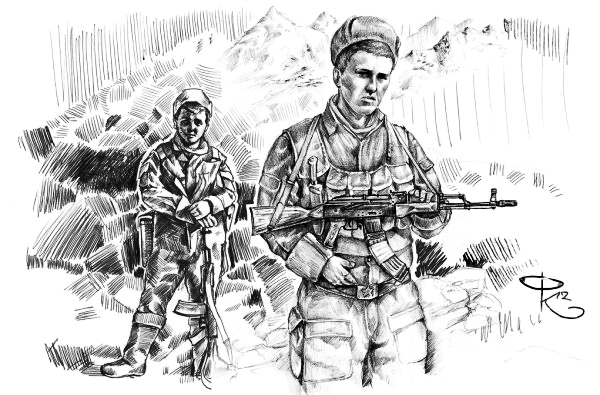
\includegraphics[scale=0.8]{img/военные.png}
\end{figure}
\newpage
\addcontentsline{toc}{subsection}{Атланты - Александр Городницкий}%В оглавление
\subsection*{Атланты}
    Ког\Em{да} на сердце \Am{тяжесть} и \CHORD{H7}{холодно} в гру\Em{ди},\\
    К ступеням Эрми\Am{тажа} ты в \CHORD{D7}{сумерки} прид\G{и},\\
    Где \CHORD{E7}{без} питья и х\Am{леба}, за\CHORD{D7}{бытые} в век\G{ах},\\
    Ат\Am{ланты} держат \Em{небо} на \CHORD{H7}{каменных} ру\CHORD{(C) Em}{ках}. (2 раза)\\
    
    \-\hspace{3mm}Держать его махину -- не мёд со стороны.\\
    \-\hspace{3mm}Напряжены их спины, колени сведены.\\
    \-\hspace{3mm}Их тяжкая работа важней иных работ:\\
    \-\hspace{3mm}Из них ослабнет кто-то -- и небо упадёт. (2 раза)\\
    
    Во тьме заплачут вдовы, повыгорят поля.\\
    И встанет гриб лиловый, и кончится Земля.\\
    А небо, год от года, всё давит тяжелей,\\
    Дрожит оно от гула ракетных кораблей. (2 раза)\\
    
    \-\hspace{3mm}Стоят они, ребята, точёные тела,\\
    \-\hspace{3mm}Поставлены когда-то, а смена не пришла.\\
    \-\hspace{3mm}Их свет дневной не радует, им ночью не до сна.\\
    \-\hspace{3mm}Их красоту снарядами уродует война. (2 раза)\\
    
    Стоят они навеки, уперши лбы в беду,\\
    Не боги -- человеки, привыкшие к труду.\\
    И жить ещё надежде до той поры, пока\\
    Атланты небо держат на каменных руках. (2 раза)
\newpage
\addcontentsline{toc}{subsection}{День победы - Давид Тухманов (ст. В. Харитонов)}%В оглавление
\subsection*{День победы}
    \Am{День} Победы, как он был от нас далёк,\\
    Как в костре потухшем таял уго\Dm{лёк}.\\
    \CHORD{E7}{Были} вёрсты, обгорелые, в пыли --\\ 
    Этот \CHORD{E7}{день} мы приближали, как могли.\\
    
    \-\hspace{10mm}\textbf{Припев:}\\
    \-\hspace{10mm}Этот \Am{День} Победы порохом \Dm{пропах},\\
    \-\hspace{10mm}Это \CHORD{E7}{праздник} с сединою на виск\F{ах}.\\
    \-\hspace{10mm}\CHORD{G9}{Это}\CHORD{A7}{ }ра\Dm{дость} со слезами на глаз\CHORD{C6 C Em7 C6}{ах}.\\
    \-\hspace{10mm}Д\H{ень} Победы! Д\E{ень} Победы! \Am{День} Победы!\\

    Дни и ночи у мартеновских печей\\
    Не смыкала наша Родина очей. \\
    Дни и ночи битву трудную вели -- \\
    Этот день мы приближали, как могли.\\

    \-\hspace{10mm}\textbf{Припев}\\

    Здравствуй, мама, возвратились мы не все...\\
    Босиком бы пробежаться по росе!\\
    Пол-Европы прошагали, пол-Земли,\\
    Этот день мы приближали, как могли.\\

    \-\hspace{10mm}\textbf{Припев}\\
\newpage
\addcontentsline{toc}{subsection}{Тёмная ночь - Марк Бернес}%В оглавление
\subsection*{Тёмная ночь}
    Am Am/C H7 E7 (2 раза)\\
    \Am{Тёмная}\CHORD{(Am/C)}{ ночь}, \Dm{только} \CHORD{G7}{пули} свист\C{ят} по степи,\\
    \Dm{Только} ветер гу\Am{дит} в проводах,\CHORD{H7}{}\\
    Тускло \CHORD{E7}{звёзды} мерц\CHORD{Am Am/C H7 E7}{ают}.\\
    В тёмную ночь ты, любимая, знаю, не спишь,\\
    И у детской кроватки тайком\\
    Ты слезу утираешь.\musVspace\\
    \-\hspace{3mm}\CHORD{A7}{Как} я люблю глубину твоих \Dm{ласковых} глаз,\\
    \-\hspace{3mm}\CHORD{G7}{Как} я хочу к ним прижаться сейч\CHORD{C Dm H7 E7}{ас} губами...\\
    \-\hspace{3mm}\Am{Тёмна}\CHORD{(Am/C)}{я ночь} \Dm{раз}дел\CHORD{G7}{яет}, люб\C{имая}, нас,\\
    \-\hspace{3mm}\Dm{И} тревожная, \Am{чёрная} степь\CHORD{H7}{}\\
    \-\hspace{3mm}Пролег\CHORD{E7}{ла} между \CHORD{Am Am/C H7 E7}{нами.}\\
    
    Верю в тебя, в дорогую подругу мою,\\
    Это вера от пули меня \\
    Тёмной ночью хранила...\\
    Радостно мне, я спокоен в смертельном бою,\\
    Знаю, встретишь с любовью меня, \\
    Что б со мной ни случилось.\musVspace\\
     \-\hspace{3mm}Смерть не страшна, с ней встречались не раз мы в степи,\\
     \-\hspace{3mm}Вот и теперь надо мною она кружится...\\
     \-\hspace{3mm}Ты меня ждёшь, и у детской кроватки не спишь,\\
     \-\hspace{3mm}И поэтому, знаю, со мной \\
     \-\hspace{3mm}Ничего не случится.
\newpage
\addcontentsline{toc}{subsection}{Журавли - Марк Бернес}%В оглавление
\subsection*{Журавли}
    Мне \Em{кажется} порою, что сол\CHORD{H7}{даты}, \\
    С кров\CHORD{H7}{авых} не пришедшие по\Em{лей},\\
    Не в \Em{землю} нашу полегли ког\CHORD{H7}{да-то},\\ 
    \CHORD{H7}{А} превратились в белых журав\Em{лей.}\\
    О\Em{ни} до сей поры с времён тех \Am{дальних} \\
    Ле\CHORD{H7}{тят}, и подают нам голо\Em{са,} \\
    Не пото\Am{му} ль так \CHORD{H7}{часто} и печ\C{ально} \\
    Мы замол\CHORD{F\musSharp7}{каем}, г\CHORD{H7}{лядя} в небе\Em{са}?\\

    \-\hspace{3mm}\-\hspace{3mm}Летит, летит по небу клин усталый,\\
    \-\hspace{3mm}\-\hspace{3mm}Летит в тумане на исходе дня,\\
    \-\hspace{3mm}\-\hspace{3mm}И в том строю есть промежуток малый, \\
    \-\hspace{3mm}\-\hspace{3mm}Быть может, это место для меня.\\
    \-\hspace{3mm}\-\hspace{3mm}Настанет день, и с журавлиной стаей \\
    \-\hspace{3mm}\-\hspace{3mm}Я поплыву в такой же сизой мгле,\\
    \-\hspace{3mm}\-\hspace{3mm}Из-под небес по-птичьи окликая \\
    \-\hspace{3mm}\-\hspace{3mm}Всех вас, кого оставил на земле.\\

    Мне кажется порою, что солдаты,\\
    С кровавых не пришедшие полей,\\
    Не в землю нашу полегли когда-то,\\
    А превратились в белых журавлей.\\
\newpage
\addcontentsline{toc}{subsection}{В землянке - К. Листов (ст. А. Сурков)}%В оглавление
\subsection*{В землянке}
    Бьётся в \Am{тесной} печ\E{урке} о\Am{гонь},\\    
    На пол\C{еньях} смол\G{а}, как слез\CHORD{C A7}{а}.\\
    И п\Dm{оёт} мне в землянке гарм\Am{онь}\\
    Про ул\E{ыбку} твою и гла\Am{за}.\\
    Про теб\G{я} мне шептали куст\C{ы}\\
    В белосн\G{ежных} полях под Москв\C{ой}.\CHORD{A7}{}\\
    Я хо\Dm{чу}, чтобы слышала \Am{ты},\\
    Как тоск\E{ует} мой голос жив\Am{ой}.\\
    
    \-\hspace{3mm}Ты теперь далеко-далеко,\\
    \-\hspace{3mm}Между нами снега и снега.\\
    \-\hspace{3mm}До тебя мне дойти нелегко,\\
    \-\hspace{3mm}А до смерти -- четыре шага.\\
    \-\hspace{3mm}Пой, гармоника, вьюге назло,\\
    \-\hspace{3mm}Заплутавшее счастье зови.\\
    \-\hspace{3mm}Мне в холодной землянке тепло\\
    \-\hspace{3mm}От твоей негасимой любви.\\
    
    Бьётся в тесной печурке огонь,\\
    На поленьях смола, как слеза.\\
    И поёт мне в землянке гармонь\\
    Про улыбку твою и глаза.
\newpage
\addcontentsline{toc}{subsection}{От героев былых времён - Р. Хозак (ст. Е. Агранович)}%В оглавление
\subsection*{От героев былых времён}
    \begin {tabline}{2}{}{}{E,A,D,G,H,E}
        \note {1}{16}{3}{2} % we use \note instead of \notel and omit the last argument
        \note {2}{9}{2}{0}
        \note {3}{9}{2}{1}
        \note {4}{9}{2}{0}
        \note {5}{9}{3}{2}
        \note {6}{9}{1}{5}
        \note {7}{9}{1}{3}
        \note {8}{9}{1}{0}
        \note {9}{9}{1}{0}
        \note {9}{9}{2}{1}
        \note {9}{9}{3}{2}
        \note {9}{9}{4}{2}
        \note {9}{9}{5}{0}
        \nextbar
        \note {1}{9}{3}{2}
        \note {2}{9}{2}{0}
        \note {3}{9}{2}{1}
        \note {4}{9}{2}{0}
        \note {5}{9}{3}{2}
        \note {6}{9}{2}{0}
        \note {7}{9}{1}{3}
        \note {8}{9}{1}{1}
        \note {9}{9}{1}{1}
        \note {9}{9}{2}{3}
        \note {9}{9}{3}{2}
        \note {9}{9}{4}{0}
    \end {tabline}
    \begin {tabline}{2}{}{}{E,A,D,G,H,E}
        \note {1}{9}{2}{0}
        \note {2}{9}{2}{1}
        \note {3}{9}{2}{3}
        \note {4}{9}{2}{1}
        \note {5}{9}{2}{0}
        \note {6}{9}{1}{0}
        \note {7}{9}{2}{3}
        \note {8}{9}{2}{0}
        \note {9}{9}{3}{1}
        \note {9}{9}{4}{2}
        \note {9}{9}{5}{2}
        \note {9}{9}{6}{0}
        \nextbar
        \note {1}{9}{2}{0}
        \note {2}{9}{2}{0}
        \note {3}{9}{2}{0}
        \note {4}{9}{3}{2}
        \note {5}{9}{2}{0}
        \note {6}{9}{2}{1}
        \note {6}{9}{5}{0}
        \note {7}{9}{3}{2}
        \note {7}{9}{4}{2}
        \note {8}{9}{5}{0}
        \note {9}{9}{6}{0}
    \end {tabline}
    От героев бы\Am{лых} времён не осталось по\Dm{рой} имён.\\                 
    Те, кто приняли с\CHORD{E7}{мертный} бой, стали просто зем\Am{лёй} и травой.\\
    Только грозная \CHORD{A7}{доблесть} их поселилась в серд\Dm{цах} живых.  \\      
    Тот Вечный ог\F{онь,} нам зав\G{ещаный} и одн\C{им}, \F{мы} в груд\CHORD{E7}{и} хран\Am{им}.\\

    \-\hspace{2mm}Погляди на моих бойцов, целый свет помнит их в лицо.\\
    \-\hspace{2mm}Вот застыл батальон в строю, снова старых друзей узнаю.\\
    \-\hspace{2mm}Хоть им нет двадцати пяти -- трудный путь им пришлось \mbox{пройти.}\\
    \-\hspace{2mm}Это те, кто в штыки поднимался, как один, те, кто брал Берлин.\\

    Нет в России семьи такой, где б не памятен был свой герой.\\
    И глаза молодых солдат с фотографий увядших глядят.\\
    Этот взгляд, словно высший суд для ребят, что сейчас растут.\\
    И мальчишкам нельзя ни солгать, ни обмануть, ни с пути \mbox{свернуть.}\\
\newpage
\addcontentsline{toc}{subsection}{Идёт солдат по городу - В. Шаинский (ст. М. Танич)}%В оглавление
\subsection*{Идёт солдат по городу}
    У сол\Am{дата} выходной, пуговицы в \Dm{ряд},\\
    Ярче с\E{олнечного} дня золотом го\Am{рят}.\\
    Часов\C{ые} на посту, в городе \Dm{весна},\\
    Проводи нас до вор\E{от}, товарищ старши\Am{на}, товарищ старшин\E{а}!\\
    \\
    \-\hspace{10mm}\textbf{Припев:}\\
    \-\hspace{10mm}Идёт солдат по \Dm{городу}, по незнакомой \Am{улице}, \\
    \-\hspace{10mm}И от улыбок д\E{евичьих} вся улица свет\Am{ла}.\\
    \-\hspace{10mm}Не обижайтесь, \Dm{девушки}, но для солдата \Am{главное},      \\
    \-\hspace{10mm}Чтобы его дал\E{ёкая} любимая жда\Am{ла}.\\
    \\
    А солдат попьёт кваску, купит эскимо,\\
    Никуда не торопясь, выйдет из кино.\\
    Карусель его помчит, музыкой звеня,\\
    И в запасе у него останется полдня, останется полдня!\\
    \\
    \-\hspace{10mm}\textbf{Припев}\\
    \\
    Где любимая живёт, липы шелестят,\\
    И садится в карусель не её солдат,\\
    Но другие ни к чему, все до одного,\\
    Если только верно ждёшь солдата своего, солдата своего!\\
    \\
    \-\hspace{10mm}\textbf{Припев}\\
\newpage
\addcontentsline{toc}{subsection}{Первым делом самолёты - ст. А. Фатьянов}%В оглавление
\subsection*{Первым делом самолёты}
    Мы -- друзь\G{я}, пере\CHORD{D7}{лётные} пт\G{ицы}.\\
    Только быт наш од\CHORD{G7}{ним} нех\C{орош},\\
    На зем\Am{ле} не ус\CHORD{E7}{пели} же\Am{ниться},\\
    А на н\C{ебе} жены не най\CHORD{D7}{дёшь}.
    \begin{gather*}
    \-\hspace{10mm}\textbf{ \textup{Припев:}}\\
    \-\hspace{10mm}\textup{Потом\G{у}, потому, что мы -- пи\Am{лоты}!}\\
    \-\hspace{10mm}\textup{Небо -- \CHORD{D7}{наш}, небо -- наш родимый д\G{ом}!}\\
    \begin{musRepeat}
    \-\hspace{10mm}\textup{Первым \CHORD{E7}{делом}, первым делом -- само\Am{лёты}\C{,}}\-\hspace{2mm}\\
    \-\hspace{10mm}\textup{Ну, а \Em{девушки}? А \CHORD{H7}{девушки} -- по\Em{том}.   }\\
    \end{musRepeat}
    \end{gather*}
    Нежный образ в душе ты голубишь,\\
    Хочешь сердце навеки отдать.\\
    Нынче встретишь, увидишь, полюбишь,\\
    А на завтра приказ улетать.\\

    \-\hspace{10mm}\textbf{Припев}\\

    Чтоб с тоскою в пути не встречаться,\\
    Вспоминая про ласковый взгляд.\\
    Мы решили, друзья, не влюбляться\\
    Даже в самых красивых девчат.\\

    \-\hspace{10mm}\textbf{Припев}\\
\newpage
\addcontentsline{toc}{subsection}{Три танкиста - Братья Покрасс (ст. Б. Ласкин)}%В оглавление
\subsection*{Три танкиста}
\vspace{-5mm}
    \begin{gather*}
    \textup{На гра\Am{нице} \Dm{тучи} ходят х\Am{муро},}\\
    \textup{Край сур\F{овый} т\E{ишиной} об\Am{ъят}.}\\
    \begin{musRepeat}
    \textup{\F{У} выс\C{оких} \CHORD{A7}{берегов} А\Dm{мура}}\\
    \textup{Часо\Am{вые} Р\E{одины} ст\Am{оят}.}\\
    \end{musRepeat}\\
    \\
    \-\hspace{3mm}\textup{Там врагу заслон поставлен прочный, }\\
    \-\hspace{3mm}\textup{Там стоит, отважен и силён, }\\
    \begin{musRepeat}
    \-\hspace{3mm}\textup{У границ земли дальневосточной }\\
    \-\hspace{3mm}\textup{Броневой ударный батальон.  }\\
    \end{musRepeat}\\
    \\
    \textup{Там живут -- и песня в том порука }\\
    \textup{Нерушимой, крепкою семьёй }\\
    \begin{musRepeat}
    \textup{Три танкиста, три весёлых друга -- }\\
    \textup{Экипаж машины боевой.  }\\
    \end{musRepeat}\\
    \\
    \-\hspace{3mm}\textup{На траву легла роса густая, }\\
    \-\hspace{3mm}\textup{Полегли туманы, широки. }\\
    \begin{musRepeat}
    \-\hspace{3mm}\textup{В эту ночь решили самураи }\\
    \-\hspace{3mm}\textup{Перейти границу у реки.  }\\
    \end{musRepeat}\\
    \\
    \textup{Но разведка доложила точно: }\\
    \textup{И пошёл, командою взметён, }\\
    \begin{musRepeat}
    \textup{По родной земле дальневосточной }\\
    \textup{Броневой ударный батальон.} 
    \end{musRepeat}
    \end{gather*}
    \newpage
    \vspace{-5mm}
    \begin{gather*}
    \textup{Мчались танки, ветер подымая, }\\
    \textup{Наступала грозная броня. }\\
    \begin{musRepeat}
    \textup{И летели наземь самураи, }\\
    \textup{Под напором стали и огня.  }\\
    \end{musRepeat}\\
    \\
    \-\hspace{3mm}\textup{И добили -- песня в том порука -- }\\
    \-\hspace{3mm}\textup{Всех врагов в атаке огневой }\\
    \begin{musRepeat}
    \-\hspace{3mm}\textup{Три танкиста, три весёлых друга -- }\\
    \-\hspace{3mm}\textup{Экипаж машины боевой!}\\
    \end{musRepeat}
    \end{gather*}\begin{spacing}{0.5}
    \end{spacing}
\addcontentsline{toc}{subsection}{Ленинградцы - И. Шварц (ст. В.Коростылёв)}%В оглавление
\subsection*{Ленинградцы}
\vspace{-5mm}
    \begin{gather*}
    \textup{В да\Am{лёком} тревожном во\E{енном} году,}\\
    \textup{Под \Dm{гром} батар\E{ей} у стра\Am{ны} на ви\CHORD{A7}{ду},}\\   
    \begin{musRepeat}
    \textup{Сто\Dm{яли} со взрослыми \Am{рядом}}\\
    \textup{Мал\Dm{ьчишки} у ст\E{ен} Ленин\Am{град}\CHORD{A7}{а}.}\-\hspace{2mm}\\
    \end{musRepeat}\\
    \\
    \-\hspace{3mm}\textup{На парте осталась раскрытой тетрадь, }\\
    \-\hspace{3mm}\textup{Не выпало им дописать, дочитать. }\\
    \begin{musRepeat}
    \-\hspace{3mm}\textup{Когда навалились на город }\\
    \-\hspace{3mm}\textup{Фугасные бомбы и голод.}\\
    \end{musRepeat}\\
    \\
    \textup{И мы никогда не забудем с тобой, }\\
    \textup{Как наши ровесники приняли бой, }\\
    \begin{musRepeat}
    \textup{Им было всего лишь тринадцать, }\\
    \textup{Но были они ленинградцы.}\\
    \end{musRepeat}\\
    \end{gather*}
\newpage
\addcontentsline{toc}{subsection}{На поле танки грохотали}%В оглавление
\subsection*{На поле танки грохотали}
    \Am{На} поле танки грохот\C{али},\\ 
    Солдаты шл\G{и} в последний б\C{ой},\\
    \CHORD{(A7)}{А} моло\Dm{дого} коман\Am{дира} \\
    Несли с проб\E{итой} голо\Am{вой}. \musVspace\\
    \-\hspace{3mm}По танку вдарила болванка, \\
    \-\hspace{3mm}Прощай, родимый экипаж. \\
    \-\hspace{3mm}Четыре трупа возле танка \\
    \-\hspace{3mm}Дополнят утренний пейзаж. \musVspace\\
    Машина пламенем объята, \\
    Вот-вот рванёт боекомплект.\\
    А жить так хочется, ребята,\\
    И вылезать уж мочи нет. \musVspace \\
    \-\hspace{3mm}Нас извлекут из-под обломков, \\
    \-\hspace{3mm}Поднимут на руки каркас.  \\
    \-\hspace{3mm}И залпы башенных орудий \\
    \-\hspace{3mm}В последний путь проводят нас. \musVspace\\
    И полетят тут телеграммы,\\
    Родных и близких известить,\\
    Что сын ваш больше не вернётся\\ 
    И не приедет погостить.\musVspace \\
    \-\hspace{3mm}В углу заплачет мать-старушка, \\
    \-\hspace{3mm}Смахнёт слезу старик отец,  \\
    \-\hspace{3mm}И молодая не узнает, \\
    \-\hspace{3mm}Какой у парня был конец.  \musVspace\\
    И будет карточка пылиться \\
    На полке пожелтевших книг,   \\
    В военной форме, при погонах, \\
    И ей он больше не жених.
\newpage
\addcontentsline{toc}{subsection}{О той весне - МультиКейс (ст. Елена Плотникова) }%В оглавление
\subsection*{О той весне}
    Кино и\Em{дёт}, воюет взв\C{од},\\
    Далёкий \Am{год} на плёнке с\CHORD{H7}{тарой}...\\
    Нелёгкий путь, ещё чуть-чуть\\
    И догорят войны пожары...\\
    Счастливый май, любимый край,\\
    Своих солдат  встречай скорее...\\
    От ран обид земля дрожит\\
    Теплом души её согреем...\\

    \-\hspace{10mm}\textbf{Припев:}\\
    \-\hspace{10mm}И в\Em{сё} о той весне ув\C{идел} я во сне,\\
    \-\hspace{10mm}При\Am{шёл} рассвет и миру улыб\CHORD{H7}{нулся},\\
    \-\hspace{10mm}Что в\Em{ьюга} отмела, что \C{верба} расцвела,\\
    \-\hspace{10mm}И пр\Am{адед} мой с вой\H{ны} домой вер\Em{нулся}...\\

    В лихом бою, в чужом краю\\
    Пусть берегут любовь и вера,\\
    Чтоб больше их пришло живых\\
    И рядовых и офицеров...\\
    Придут весной, как прадед мой,\\
    И в дом родной откроют двери...\\
    Я помню свет далёких лет,\\
    В свою страну я буду верить...\\

    \-\hspace{10mm}\textbf{Припев (2 раза)}\\
\newpage
\addcontentsline{toc}{subsection}{Песня 10-го десантного батальона - Б. Окуджава}%В оглавление
\subsection*{Песня 10-го десантного батальона}
    \Am{Здесь} п\CHORD{E7}{тицы} не по\Am{ют}, де\CHORD{E7}{ревья} не рас\Am{тут},\\
    \CHORD{E7}{И} только м\E{ы} пле\CHORD{E7}{чом} к плечу врастаем в з\E{емлю} \Am{тут}.\\
    \Am{Горит} и к\CHORD{E7}{ружится} пла\Am{нета}, \Dm{над} нашей р\A{одиною} \Dm{дым},\\
    И, значит, \CHORD{G7}{нам} нужна одна поб\C{еда},\\                   
    Одна на в\CHORD{H7}{сех} -- мы за це\CHORD{E7}{ной} не посто\Am{им}. (2 раза)\musVspace\\
    \-\hspace{10mm}\textbf{Припев:}\\
    \-\hspace{10mm}\CHORD{G7}{Нас} жд\C{ёт} о\CHORD{G7}{гонь} смерт\C{ельный},\\
    \-\hspace{10mm}И в\CHORD{E7}{сё} ж\E{ }бессилен \F{он}:\\
    \-\hspace{10mm}Сомненья п\Dm{рочь}, уходит в \CHORD{G7}{ночь} отд\C{ельный}\\
    \-\hspace{10mm}Дес\E{ятый} наш де\CHORD{E7}{сантный} батал\Am{ьон}. (2 раза)\musVspace\\
    Едва огонь погас, звучит другой приказ.\\
    И почтальон сойдёт с ума, разыскивая нас.\\
    Взлетает красная ракета, бьёт пулемет, неутомим,\\
    И, значит, нам нужна одна победа, \\
    Одна на всех -- мы за ценой не постоим. (2 раза) \musVspace\\
    \musVspace
    \-\hspace{10mm}\textbf{Припев}\\
    От Курска и Орла война нас довела\\
    До самых вражеских ворот, такие, брат, дела.\\
    Когда-нибудь мы вспомним это, и не поверится самим,\\
    А нынче нам нужна одна победа, \\
    Одна на всех -- мы за ценой не постоим. (2 раза)\musVspace\\
    \-\hspace{10mm}\textbf{Припев}
\newpage

\addcontentsline{toc}{section}{Походные песни}%В оглавление
\section*{\centerline{Походные песни}}
\vspace{10mm}
\begin{figure}[h]
       \centering
        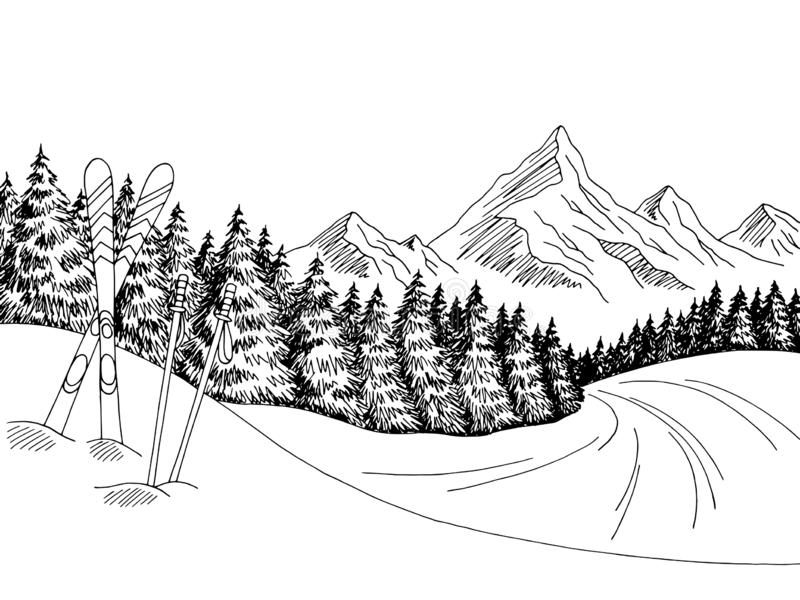
\includegraphics[scale=1.8]{img/походные.jpg}
\end{figure}
\newpage
\addcontentsline{toc}{subsection}{Вершина - Владимир Высоцкий}%В оглавление
\subsection*{Вершина}
\vspace{-5mm}
    \begin{gather*}
    \textup{Зд\Cm{есь} вам не равнина -- здесь климат иной.}\\
    \textup{Ид\Cm{ут} лавины одна за одной,}\\
    \textup{И з\Fm{десь} за камне\CHORD{A\musSharp7}{падом} ревёт камнеп\CHORD{D\musSharp}{ад}.\CHORD{C7}{}}  \\
    \textup{И м\Fm{ожно} свернуть, обрыв обогнуть,}\\
    \begin{musRepeat}
    \textup{Но \Cm{мы} выбираем трудный путь,}\\
    \textup{Оп\CHORD{G7}{асный}, как во\CHORD{A\musSharp{}m}{енная} тропа. }\\
    \end{musRepeat}\\
    \\
    \-\hspace{3mm}\textup{Кто здесь не бывал, кто не рисковал,}\\
    \-\hspace{3mm}\textup{Тот сам себя не испытал,}\\
    \-\hspace{3mm}\textup{Пусть даже внизу он звёзды хватал с небес.}\\
    \-\hspace{3mm}\textup{Внизу не встретишь, как не тянись,}\\
    \begin{musRepeat}
    \-\hspace{3mm}\textup{За всю свою счастливую жизнь}\\
    \-\hspace{3mm}\textup{Десятой доли таких красот и чудес. }\\
    \end{musRepeat}\\
    \\
    \textup{Нет алых роз и траурных лент,}\\
    \textup{И не похож на монумент}\\
    \textup{Тот камень, что покой тебе подарил.}\\
    \textup{Как Вечным огнём, сверкает днём}\\
    \begin{musRepeat}
    \textup{Вершина изумрудным льдом,}\\
    \textup{Которую ты так и не покорил. }
    \end{musRepeat}\\
    \end{gather*}
    \newpage
    \begin{gather*}
    \textup{И пусть говорят -- да, пусть говорят!}\\
    \textup{Но нет -- никто не гибнет зря,}\\
    \textup{Так -- лучше, чем от водки и от простуд!}\\
    \textup{Другие придут, сменив уют}\\
    \begin{musRepeat}
    \textup{На риск и непомерный труд, -- }\\ 
    \textup{Пройдут тобой не пройденный маршрут. }\\
    \end{musRepeat}\\
    \\
    \-\hspace{3mm}\textup{Отвесные стены -- а ну, не зевай!}\\
    \-\hspace{3mm}\textup{Ты здесь на везение не уповай.}\\
    \-\hspace{3mm}\textup{В горах ненадёжны ни камень, ни лёд, ни скала.}\\
    \-\hspace{3mm}\textup{Надеемся только на крепость рук,}\\
    \begin{musRepeat}
    \-\hspace{3mm}\textup{На руки друга и вбитый крюк,}\\
    \-\hspace{3mm}\textup{И молимся, чтобы страховка не подвела. }\\
    \end{musRepeat}\\
    \\
    \textup{Мы рубим ступени... Ни шагу назад!}\\
    \textup{И от напряженья колени дрожат,}\\
    \textup{И сердце готово к вершине бежать из груди.}\\
    \textup{Весь мир на ладони! Ты счастлив и нем,}\\
    \begin{musRepeat}
    \textup{И только немного завидуешь тем, }\\
    \textup{Другим -- у которых вершина ещё впереди. }\\
    \end{musRepeat}\\
    \end{gather*}
\newpage
\addcontentsline{toc}{subsection}{Перевал - Юрий Визбор}%В оглавление
\subsection*{Перевал}
    \Am{Просто} нечего нам б\Dm{ольше} терять.\CHORD{E7}{}\\
    Всё нам вспомнится на стр\Am{ашном} суде.\\  
    Эта ночь легла как т\Dm{от} перевал,\G{  }\\
    За которым исполн\C{ение} надежд.\CHORD{A7}{} \\
    Просто прожитое пр\Dm{ожито} зря, не зря,\G{  }\\
    Но не в этом, поним\C{аешь} ли, соль.\Am{ }\\
    Слышишь, падают дожд\Dm{и} октября,\CHORD{E7}{}\\
    Видишь, старый дом сто\Am{ит} средь лесов. \\
    
    \-\hspace{3mm}Мы затопим в доме печь, в доме печь, \\
    \-\hspace{3mm}Мы гитару позовём со стены.\\
    \-\hspace{3mm}Просто нечего нам больше беречь,\\
    \-\hspace{3mm}Ведь за нами все мосты сожжены,\\
    \-\hspace{3mm}Все мосты, все перекрёстки дорог,\\
    \-\hspace{3mm}Все прошёптанные тайны ночи.\\
    \-\hspace{3mm}Каждый сделал всё что смог, всё что смог.\\
    \-\hspace{3mm}Но об этом помолчим, помолчим.\\
    \newpage
    И луна взойдёт оплывшей свечой,\\
    Ставни скрипнут на ветру, на ветру,\\
    Ах, как я тебя люблю да горячо,\\
    Годы это не сотрут, не сотрут.\\
    Мы оставшихся друзей соберём,\\
    Мы набьём картошкой старый рюкзак,\\
    Люди спросят: ``Что за шум, что за гам?'',\\
    Мы ответим: ``Просто так, просто так''.

    \-\hspace{3mm}Просто так идут дожди октября,\\
    \-\hspace{3mm}И потеряны от счастья ключи.\\
    \-\hspace{3mm}Это всё конечно мне, конечно мне,\\
    \-\hspace{3mm}Но об этом помолчим, помолчим,\\
    \-\hspace{3mm}Просто прожитое прожито зря, не зря,\\
    \-\hspace{3mm}Но не в этом, понимаешь ли, соль,\\
    \-\hspace{3mm}Слышишь, падают дожди октября,\\
    \-\hspace{3mm}Видишь, старый дом стоит средь лесов.\begin{spacing}{0.5}
    \end{spacing}
\newpage
\addcontentsline{toc}{subsection}{Лесные леди - Нелли Путина}%В оглавление
\subsection*{Лесные леди}\begin{spacing}{0.5}
\end{spacing}
    Кто-то с\Am{кажет} с усм\Em{ешкой}: ``Ну, \Am{надо} же, \\
    Девч\F{онки}, а в\Em{сё} ту\Am{да} же!'' \\
    И распишут в кр\Em{асках} не\Am{радужных}\\ 
    Этот п\F{уть}, чуть о\Em{пасный} \Am{даже}.\\
    Но ко\Dm{го} бы пуг\G{али}! Зн\C{аете}?\\ 
    Разве \Dm{им} это вс\E{ё} в\Am{ажно}\CHORD{A7}{.} \\
    Они с\Dm{вязаны} с \G{этим} \C{намерт}\Am{во}, \\
    Свой \Dm{выбор} сд\E{елав} од\Am{нажды}.\musVspace\\
    \-\hspace{10mm}\textbf{Припев:}\\
    \-\hspace{10mm}Лесные \Dm{леди}, ч\G{удо} из всех чуд\C{ес}.\\ 
    \-\hspace{10mm}Принцессы \Dm{шумных} пал\E{аточных} коро\Am{левств}\CHORD{A7}{.}\\
    \-\hspace{10mm}Из звёзд, из \Dm{солнца}, из р\G{адуг} и летних гр\C{оз},\\
    \-\hspace{10mm}Лесные \Dm{леди}. Ф\E{еи} утренних \Am{рос}. \musVspace\\
    И опять в электричку первую, \\
    С рюкзаками наперевес, \\
    Выбирая дорогу верную. \\
    Вам -- курорты, а им -- лес! \\
    Чтобы вновь вечерами длинными,\\ 
    Под звёздным ночным шатром \\
    Петь песни свои любимые, \\
    Согреваясь одним костром.
    \newpage
    \-\hspace{10mm}\textbf{Припев}\\
    Ни о чём не решаете загодя,\\
    Не хлебнув родниковых вод,\\
    Из окон квартир не понять,\\
    Куда та лесная тропа ведёт,\\
    Чем влечёт их река бурлящая,\\
    Что слышится в пенье птиц, \\
    Что за сказка, так их манящая \\
    За черту городских границ?\musVspace\\
    \-\hspace{10mm}\textbf{Припев}\begin{spacing}{0.5}\end{spacing}
\addcontentsline{toc}{subsection}{Люди идут по свету - Р. Ченборисова (ст. И. Сидоров)}%В оглавление
\subsection*{Люди идут по свету}
\vspace{-5mm}
    \begin{gather*}
    \textup{\Am{Люди} идут по св\Dm{ету}, им, вр\E{оде}, немного н\Am{адо}: }\\
    \textup{Была бы прочна пал\Dm{атка} и б\CHORD{G7}{ыл} бы нескучен п\C{уть}. }\\
    \begin{musRepeat}
    \textup{Hо с д\CHORD{A7}{ымом} сливается п\Dm{есня}, реб\CHORD{G7}{ята} отводят взгл\C{яды},} \\
    \textup{И ш\Am{епчет} во сне брод\Dm{яга} ком\E{у-то}: ``Hе позаб\Am{удь}!''}\musVspace\\
    \end{musRepeat}\\
    \-\hspace{3mm}\textup{Они в городах не блещут манерами аристократов, }\\
    \-\hspace{3mm}\textup{Hо в чутких концертных залах, где шум суеты затих, }\\
    \begin{musRepeat}
    \-\hspace{3mm}\textup{Страдают в бродячих душах бетховенские сонаты, }\\
    \-\hspace{3mm}\textup{И светлые песни Грига переполняют их.} \musVspace\\
    \end{musRepeat}\\
    \textup{А люди идут по свету, слова их порою грубы. }\\
    \textup{``Пожалуйста'', ``извините'', -- с усмешкой они говорят.  }\\
    \begin{musRepeat}
    \textup{Но грустную нежность песни ласкают сухие губы, }\\
    \textup{И самые лучшие книги они в рюкзаках хранят.}\musVspace\\
    \end{musRepeat} \\
    \-\hspace{3mm}\textup{Выверен старый компас, получены карты в сроки, }\\
    \-\hspace{3mm}\textup{И выштопан на штормовке лавины предательский след. }\\
    \begin{musRepeat}
    \-\hspace{3mm}\textup{Счастлив, кому знакомо щемящее чувство дороги, }\\
    \-\hspace{3mm}\textup{Где ветер рвет горизонты и раздувает рассвет.}
    \end{musRepeat}\\
    \end{gather*}
\newpage
\addcontentsline{toc}{subsection}{Дым костра - Александр Евстигнеев}%В оглавление
\subsection*{Дым костра}
\vspace{-5mm}
    \begin{gather*}
    \textup{\Am{Дым} костра созда\Dm{ёт} уют,}\\
    \textup{\G{Искры} гаснут в пол\C{ёте} сами,}\\
    \begin{musRepeat}
    \textup{\Dm{Пять} ребят о люб\Am{ви} поют,}\\
    \textup{Ч\E{уть} охрипшими \Am{голосами}. }\\
    \end{musRepeat}\\
    \\
    \-\hspace{3mm}\textup{Пять сердец бьются как одно,}\\
    \-\hspace{3mm}\textup{Вспоминая подруг далёких,}\\
    \begin{musRepeat}
    \-\hspace{3mm}\textup{Тех, что ждут их уже давно, }\\
    \-\hspace{3mm}\textup{Самых близких и яснооких.}\\
    \end{musRepeat}\\
    \\
    \textup{Если б слышали те, о ком,}\\
    \textup{Эта песня сейчас звучала,}\\
    \begin{musRepeat}
    \textup{Прибежали б сюда тайком,}\\
    \textup{Чтоб послушать её с начала. }\\
    \end{musRepeat}\\
    \\
    \-\hspace{3mm}\textup{Чтоб почувствовать до конца,}\\
    \-\hspace{3mm}\textup{Эти губы и эти руки,}\\
    \begin{musRepeat}
    \-\hspace{3mm}\textup{Как умеют любить сердца, }\\
    \-\hspace{3mm}\textup{Огрубевшие от разлуки.}\\
    \end{musRepeat}\\
    \\
    \textup{Дым костра создаёт уют,}\\
    \textup{Искры гаснут в полёте сами,}\\
    \begin{musRepeat}
    \textup{Пять ребят о любви поют,}\\
    \textup{Чуть охрипшими голосами. }\\
    \end{musRepeat}\\
    \end{gather*}
\newpage
\addcontentsline{toc}{subsection}{Изгиб гитары жёлтой - Олег Митяев}%В оглавление
\subsection*{Изгиб гитары жёлтой}
\vspace{-5mm}
    \begin{gather*}
    \textup{Из\Am{гиб} гитары \Dm{жёлтой} ты обн\CHORD{E7}{имешь} \Am{нежно},}\\
    \textup{Стру\Am{на} осколком \Dm{эха} пронз\G{ит} тугую в\C{ысь},}\\
    \begin{musRepeat}
    \textup{Кач\CHORD{A7}{нётся} купол \Dm{неба} больш\G{ой} и звёздно-с\C{нежный},}\\
    \textup{Как з\Dm{дорово,} что в\Am{се} мы здесь сег\E{одня} собрал\CHORD{F (Am)}{ись}.}\hspace{3mm}\\
    \end{musRepeat}\\
     \\
    \-\hspace{3mm}\textup{Как отблеск от заката костёр меж сосен скачет,}\\
    \-\hspace{3mm}\textup{Ну, что грустишь, бродяга, а ну-ка улыбнись.}\\
    \begin{musRepeat}
    \-\hspace{3mm}\textup{И кто-то очень близкий тебе тихонько скажет:}\\
    \-\hspace{3mm}\textup{Как здорово, что все мы здесь сегодня собрались.}\\
    \end{musRepeat}\\
    \\
    \textup{И всё же с болью в горле мы тех сегодня вспомним,}\\
    \textup{Чьи имена как раны на сердце запеклись.}\\
    \begin{musRepeat}
    \textup{Мечтами их и песнями мы каждый вздох наполним.}\\
    \textup{Как здорово, что все мы здесь сегодня собрались. }\\
    \end{musRepeat}\\
    \\
    \-\hspace{3mm}\textup{Изгиб гитары жёлтой ты обнимешь нежно,}\\
    \-\hspace{3mm}\textup{Струна осколком эха пронзит тугую высь, }\\
    \begin{musRepeat}
    \-\hspace{3mm}\textup{Качнётся купол неба большой и звёздно-снежный,}\\
    \-\hspace{3mm}\textup{Как здорово, что все мы здесь сегодня собрались. }\\
    \end{musRepeat}\\
    \end{gather*}
\newpage
\addcontentsline{toc}{subsection}{Русская дорога - Игорь Растеряев}%В оглавление
\subsection*{Русская дорога}
    По п\Am{лачущей} земле, не чуя сапогов,\\
    Наш \Am{обескровленный} отряд уходит от врагов,\\
    Пи\Dm{таясь} на ходу щавелевым листом,\\
    Ноч\F{уя} в буераке под кал\E{иновым} кустом.\\
    Нам отдохнуть нельзя, бегом-бегом-бегом,\\
    А наши ``якобы друзья'' засели за бугром\\
    И смотрят, как нас бьют, не отрывая глаз,\\
    И только длинные дороги полностью за нас!\\
    \-\hspace{10mm}\Dm{Вытри} слезы, \E{отдохни} нем\Am{ного.} Я -- русская дорога!\CHORD{Dm E Am}{}\\
    \-\hspace{10mm}Отходи, а я тебя прикрою грязью, да водою.\musVspace\\
    Но по уши в грязи, в воде до самых глаз,\\
    Через какой-то срок враги опять нагнали нас\\
    И бьют ещё сильней, вот-вот и порешат,\\
    Но лютые морозы к нам на выручку спешат!\musVspace\\
    \-\hspace{10mm}Отдохни, утри горючи слёзы. Мы -- русские морозы.\\
    \-\hspace{10mm}Заморозим, заметём тоскою, поманив Москвою.\musVspace\\
    Природа на войне нам как родная мать,\\
    Но есть время хорониться, а есть время наступать,\\
    И скоро объявились мы во вражьих городках,\\
    И стали всё крушить вокруг, разбили в пух и прах.\\
    Порвали на куски, размолотили в хлам,\\
    И добивая, объясняли стонущим врагам:\\
    ``Запомните загадочный тактический приём:\\
    Когда мы отступаем -- это мы вперёд идём!''\musVspace\\
    \-\hspace{10mm}Вместе с холодами и лесами. Впереди Сусанин.\\
    \-\hspace{10mm}Просто нам завещана от Бога русская дорога.
 \newpage
\addcontentsline{toc}{section}{Начинающим}%В оглавление
\section*{\centerline{Начинающим}}
\addcontentsline{toc}{subsection}{Советы опытных гитаристов}%В оглавление
\subsection*{Советы опытных гитаристов}
\begin{itemize}
  \item Открывайте шире рот, когда поёте. Исполнение песен под гитару -- это умение не только играть, но и петь. Регулярно делайте артикуляционную гимнастику.
  \item Следите за темпом. Вначале вы будете медленно переставлять аккорды и со временем научитесь делать это быстрее. Если вы умеете переставлять аккорды быстро, то не значит, что нужно это делать. Не ускоряйте песню. 
  \item Не бойтесь сложных аккордов. Если вы увидели страшный  аккорд A9sus4/H и не знаете, как его играть, отбросьте всё лишнее и сыграйте A. Однако стоит выучить несыгранный сложный аккорд, и в будущем ваша игра станет красивее и ярче. Также это касается dim, 5, 6, +, sus2, sus4, maj7.
  \item Если нет каподастра или медиатора, можно справиться подручными средствами. Каподастр легко делается из карандаша и резинки (канцелярской или для волос). Для медиатора подойдёт любой тонкий удобный предмет. Лучше не использовать металл (легко порвать струны).
  \item Мозоли на левой руке -- на самом деле ваши друзья. Первые недели непривыкшие пальцы будут болеть, но со временем кожа огрубеет и пальцы привыкнут играть часами. В начале пути лучше играть на мягких нейлоновых струнах. Нужно играть часто, но не долго.
  \item Если вы не знаете бой или плохо справляетесь с ритмом, обычный ``трунь'' вниз на каждый аккорд уже достаточен, чтобы петь песню. Чаще всего аккорды меняются на гласных буквах. При уверенных ``трунях'' на каждый аккорд можно добавлять дополнительные и экспериментировать.
  \item Весь успех в регулярности. Со временем пальцы сами всё запоминают. Любите гитару и продолжайте, даже если не сразу получается!
\end{itemize}
\newpage
\addcontentsline{toc}{subsection}{Гитара и постановка рук}%В оглавление
\subsection*{Гитара и постановка рук}
\begin{figure}[h]
       \centering
        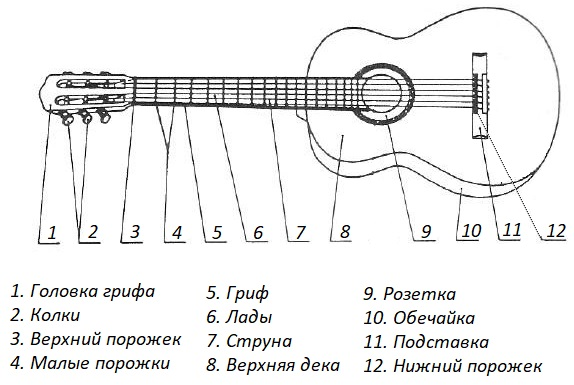
\includegraphics[scale=1.10]{other/гитара.jpg}
\end{figure}
\begin{tabular}{cc} 
   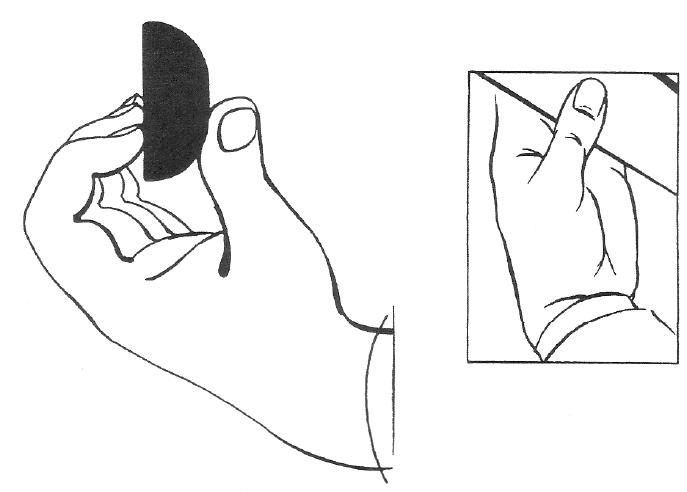
\includegraphics[scale=0.45]{other/руки.jpg}&
   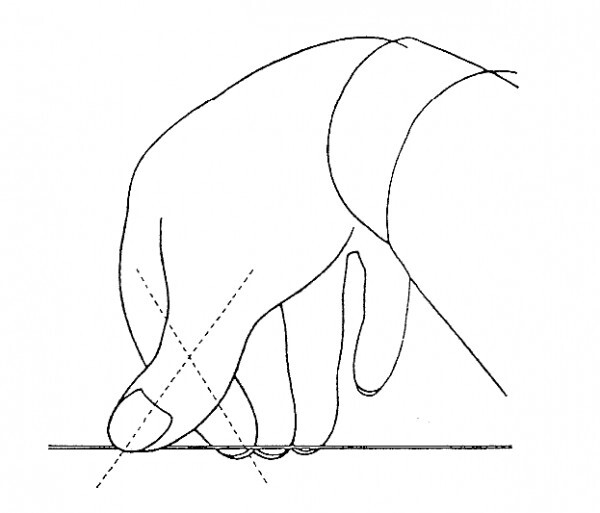
\includegraphics[scale=0.25]{other/руки2.jpg}\\
   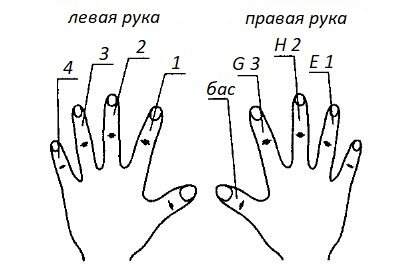
\includegraphics[scale=0.40]{other/руки3.jpg}&
   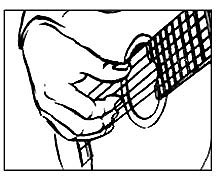
\includegraphics[scale=0.55]{other/руки4.jpg}\\
\end{tabular}
\newpage
\textbf{Правая рука} должна быть расслаблена и свободно висеть напротив розетки. При ударе по струнам вниз задействуется весь большой палец.\\
Большой палец \textbf{левой руки} должен упираться в гриф или же немного его обхватывать (при игре на высоких струнах). 
Каждому пальцу левой руки соответствуют номера. Их пишут на схемах аккордов. Большой палец не задействуется. Для правой руки при игре перебором, на каждый палец приходится своя струна: большому три басовые (4-6), а указательному, среднему и безымянному -- струны 3,2,1. \begin{spacing}{0}\end{spacing}
\addcontentsline{toc}{subsection}{Теория}%В оглавление
\subsection*{Теория}
Аккорд -- одновременное сочетание трёх и более звуков (нот). \\
Каждой основной ноте соответствует своя буква. Обратите внимание, что ряд зацикливается и снова начинается с ``до''.\\

\begin{tabular}{|c|c|c|c|c|c|c|c|}
\hline
C & D & E & F & G & A & H & C\\
до & ре & ми & фа & соль & ля & си & до\\
\hline
\end{tabular}\\

Аккорд называют по его главной ноте.\\
Аккорды бывают мажорные и минорные. Мажорные аккорды обозначаются заглавными латинскими буквами (\textbf{A -- ля мажор}). Минорные аккорды по звучанию более спокойные и обозначаются маленькой буквой \textbf{m} (\textbf{Am -- ля минор}). Также существуют септаккорды, они обозначаются цифрой 7 \textbf{(A7 -- ля мажорный септаккорд)}. Ноты можно повышать и понижать. Знак \musSharp{}~(\textbf{диез}) поднимает ноту на полтона выше, а b (\textbf{бемоль}) опускает её. \mbox{Полтона} -- наименьшее расстояние между звуками в музыке. \\Аккорды с такими знаками обозначаются:\\\textbf{A\musSharp{} -- ля диез мажор} и \textbf{Ebm -- ми бемоль минор.}\\

\begin{tabular}{|c|c|c|c|c|c|c|c|c|c|c|c|c|}
\hline
\textbf{C} & C\musSharp & \textbf{D} & D\musSharp & \textbf{E} & \textbf{F} & F\musSharp & \textbf{G} & G\musSharp & \textbf{A} & A\musSharp & \textbf{H} & \textbf{C} \\
\textbf{C} & Db & \textbf{D} & Eb & \textbf{E} & \textbf{F} & Gb & \textbf{G} & Ab & \textbf{A} & Hb & \textbf{H} & \textbf{C}\\
\hline
\end{tabular}\\

Обратите внимание, что между некоторыми основными нотами нет промежуточных. Точно так же, как на пианино, между некоторыми белыми клавишами нет чёрных. Промежуточных нот нет между E-F и между H-C.
Таким образом \textbf{E\musSharp{} = F} и \textbf{Cb = H}.
\newpage
\addcontentsline{toc}{subsection}{Устройство струн и ладов}%В оглавление
\subsection*{Устройство струн и ладов}
\textbf{Струны} на гитаре считаются снизу вверх -- от самой тонкой до самой толстой. \\
\textbf{Лады} считаются, начиная от порожка до конца грифа. На некоторых гитарах стоят специальные точки для упрощения их поиска. Один лад -- один полутон.\vspace{7mm}\\
\setchordscheme{rotate = 180, name-distance = 0mm, tuning ={1 струна -- E(Ми), 2 струна -- H(Си), 3 струна -- G(Соль), 4 струна -- D(Ре), 5 струна -- A(Ля), 6 струна -- E(Ми)},  name-below = true, name-format = {\large\selectfont},  restrict-bounding-box = true, finger-y-offset = {0.4},finger-x-offset = {0},finger-radius = {0}}
\muschordscheme[
name = $\leftarrow$розетка |  колки$\rightarrow$,
finger    = {1/6:I лад, 2/6:II лад, 3/6:III лад, 4/6:IV лад},
]\\
\\
\textbf{Как настроить гитару}\\
\\
Для этого нужно специальное приложение на телефоне или небольшое устройство (тюнер), которое крепится прямо на гитару. Вам нужно дёрнуть струну, а устройство покажет как сильно стоит подтянуть колок. Делать это нужно не спеша, следя за стрелкой тюнера.\\
Если тюнера нет, то воспользуйтесь фактом, что одну и ту же ноту можно зажать в нескольких местах гитары. Вся настройка должна быть от первой струны по порядку. На слух подкручивайте колки, чтобы струны звучали одинаково.\\
Зажатая на 5 ладу 2-я струна должна звучать как открытая 1-я\\
Зажатая на 4 ладу 3-я -- как открытая 2-я; \\
Зажатая на 5 ладу 4-я -- как открытая 3-я; \\
Зажатая на 5 ладу 5-я -- как открытая 4-я; \\
Зажатая на 5 ладу 6-я -- как открытая 5-я;\\

\newpage
\begin{figure}
    \centering
    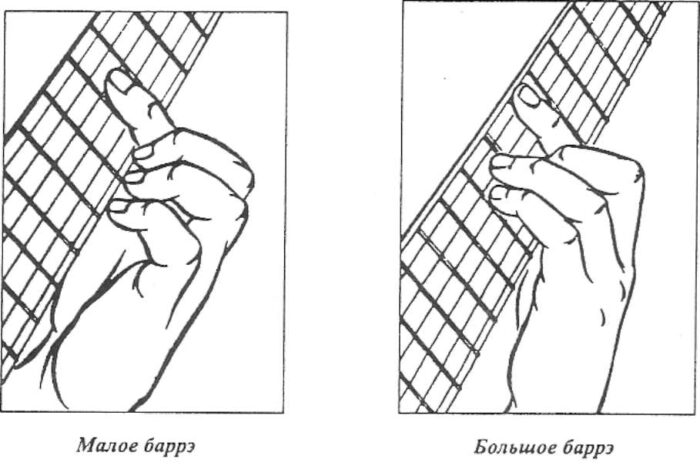
\includegraphics[scale=0.90]{other/баррэ.jpg}
\end{figure}
\textbf{Баррэ}\\
Палец должен находиться ровно вдоль лада и одновременно прижимать все струны широкой частью. Если какая-то струна не будет прижата, то она не будет звучать, или будет издавать глухой звук.\\
Уделите особое внимание положению большого пальца. Он должен быть прижат к грифу с обратной стороны. Подушечка должна упираться в середину грифа или располагаться немного выше, если у вас длинные пальцы.\\

\textbf{Как читать табулатуры}
\begin{tabline}{1}{}{}{E,A,D,G,H,E}
\note{1}{8}{5}{0}
\note{2}{8}{3}{2}
\note{3}{8}{2}{1}
\note{4}{8}{3}{2}
\note{5}{8}{1}{0}
\note{6}{8}{3}{2}
\note{7}{8}{2}{1}
\note{8}{8}{3}{2}
\end{tabline}
На данной схеме изображён гриф гитары, нумерация струн ставится сверху вниз, т.е. самая верхняя -- это первая, нижняя -- шестая. На каждой струне числами обозначены лады, которые необходимо зажать. Их нужно читать последовательно. Если числа находятся друг под другом, их нужно играть одновременно. В данном примере представлен перебор восьмёрка при зажатом аккорде Am.\\
\newpage

\addcontentsline{toc}{section}{Справочные материалы}%В оглавление
\section*{\centerline{Справочные материалы}}
\addcontentsline{toc}{subsection}{Бои}%В оглавление
\subsection*{Бои}
\textbf{Четвёрка:}\musVspace\\
\scalebox{2}{$\mathsf{\downarrow\hspace{1.5mm}\uparrow{}X\uparrow}$}\musVspace\\
\textit{стр 4} Земной простор (вместо первого $\downarrow$ можно щипок баса)\\
\textit{стр 32} Звезда по имени солнце (немного изменён $\mathsf{\downarrow\hspace{0.75mm}\uparrow{}X\uparrow\hspace{0.75mm}\downarrow\hspace{0.75mm}\uparrow{}X\_}$)\\
\textit{стр 84} Вершина\\

\textbf{Шестёрка с глушением}\musVspace\\
\scalebox{2}{$\mathsf{\downarrow{}\_X\uparrow\_\uparrow{}X\uparrow}$}\musVspace\\
\textit{стр 2} Будь готов\\
\textit{стр 14} Что такое осень\\
\textit{стр 44} Землю обмотали\\
\textit{стр 68} Перевал\\

\textbf{Шестёрка}\musVspace\\
\scalebox{2}{$\mathsf{\downarrow\_\downarrow\hspace{1.5mm}\uparrow\_\uparrow\hspace{1.5mm}\downarrow\hspace{1.5mm}\uparrow}$}\musVspace\\
\textit{стр 16} Этот город \\
\textit{стр 25} Дыхание\\
\textit{стр 43} Алые паруса\\

\textbf{Восьмёрка}\musVspace\\
\scalebox{2}{$\mathsf{\downarrow\_\_\_\downarrow\_\_\_\uparrow\_\uparrow\_\downarrow\downarrow\downarrow\uparrow}$}\musVspace\\
\textit{стр 9} Костёр\\
\textit{стр 24} Сансара
\newpage
\addcontentsline{toc}{subsection}{Переборы}%В оглавление
\subsection*{Переборы}
\textbf{Перебор шестёрка}\musVspace\\
\textbf{Б-3-2-1-2-3}\musVspace\\
\textit{стр 36} Алые паруса - В. Ланцберг\\
\textit{стр 55} Журавли\\

\textbf{Перебор восьмёрка}\musVspace\\
\textbf{Б-3-2-3-1-3-2-3}\musVspace\\
\textit{стр 8} Мой рок-н-ролл\\
\textit{стр 18} Ты неси меня река\\

\textbf{Перебор щипковый}\musVspace\\
\textbf{Б-123}\musVspace\\
\textit{стр 47} Большой секрет\\
\textit{стр 49} Дружба крепкая\\
\textit{стр 50} В каждом маленьком ребёнке\\
\textit{стр 58} Идёт солдат по городу\\

\textbf{Перебор щипковый вальсовый}\musVspace\\
\textbf{Б-123-123}\musVspace\\
\textit{стр 56} В землянке\\
\textit{стр 71} Люди идут по свету\\
\newpage
\setchordscheme{rotate = -90, name-distance = 0mm, tuning ={E, H, G, D, A, E},  name-below = true, name-format = {\large\fontseries{bx}\selectfont}, restrict-bounding-box = true, finger-y-offset = {0.4},finger-x-offset = {0.3},finger-radius = {.1875}}
\addcontentsline{toc}{subsection}{Схемы аккордов}%В оглавление
\muschordscheme[
name      = C ,
position  = I,
finger    = {1/2:1, 3/5:3, 2/4:2},
ring      = {5},
mute = {6}
]
\muschordscheme[
name      = Cm ,
position  = III,
barre = 1/1-5: ,
finger    = {2/2:2, 3/3:4, 3/4:3},
ring      = {5},
mute = {6}
]
\muschordscheme[
name      = C7,
position  = I,
finger    = {1/2:1, 3/5:3, 2/4:2, 3/3:4},
ring      = {5},
mute = {6}
]\vspace{7mm}\\
\muschordscheme[
name      = D,
position  = I,
finger    = {2/3:1, 2/1:2, 3/2:3},
ring      = {4},
mute = {6,5}
]
\muschordscheme[
name      = Dm,
position  = I,
finger    = {1/1:1, 2/3:2, 3/2:4},
ring      = {4},
mute = {6,5}
]
\muschordscheme[
name      = D7,
position  = I,
finger    = {2/3:2, 2/1:3, 1/2:1},
ring      = {4},
mute = {6,5}
]\vspace{7mm}\\
\muschordscheme[
name      = E,
position  = I,
finger    = {1/3:1, 2/4:3, 2/5:2},
ring      = {6},
]
\muschordscheme[
name      = Em,
position  = I,
finger    = { 2/4:3, 2/5:2},
ring      = {6},
]
\muschordscheme[
name      = E7,
position  = I,
finger    = {1/3:1,  2/5:2, 3/2:4},
ring      = {6},
]\vspace{7mm}
                                \newpage
\muschordscheme[
name      = F,
position  = I,
barre = 1/1-6:,
finger    = {2/3:2, 3/4:4, 3/5:3},
ring      = {6},
]
\muschordscheme[
name      = Fm,
position  = I,
barre = 1/1-6:,
finger    = { 3/4:3, 3/5:2},
ring      = {6},
]
\muschordscheme[
name      = F7,
position  = I,
barre = 1/1-6:,
finger    = {2/3:2,  3/5:3, 4/2:4},
ring      = {6},
]\vspace{7mm}\\
\muschordscheme[
name      = G,
position  = I,
finger    = {2/5:2, 3/6:3, 3/1:4},
ring      = {6},
]
\muschordscheme[
name      = Gm,
position  = III,
barre = 1/1-6:,
finger    = { 3/4:3, 3/5:2},
ring      = {6},
]
\muschordscheme[
name      = G7,
position  = I,
finger    = {2/5:2,  3/6:3, 1/1:1},
ring      = {6},
]\vspace{7mm}\\
\muschordscheme[
name      = A ,
position  = I,
finger    = {2/2:3, 2/3:2, 2/4:1},
ring      = {5},
mute = {6}
]
\muschordscheme[
name      = Am ,
position  = I,
finger    = {1/2:1, 2/3:3, 2/4:2},
ring      = {5},
mute = {6}
]
\muschordscheme[
name      = A7,
position  = I,
finger    = {2/2:3, 2/4:2},
ring      = {5},
mute = {6}
]\vspace{7mm}   
                            \newpage
\muschordscheme[
name      = H,
position  = II,
barre = 1/1-5: ,
finger    = {3/2:4, 3/3:3, 3/4:2},
ring      = {5},
mute = {6}
]
\muschordscheme[
name      = Hm,
position  = II,
barre = 1/1-5: ,
finger    = {2/2:2, 3/3:4, 3/4:3},
ring      = {5},
mute = {6}
]
\muschordscheme[
name      = H7,
position  = I,
finger    = {1/4:1, 2/5:2, 2/3:2,2/1:1},
ring      = {5},
mute = {6}
]\vspace{7mm}\\
\muschordscheme[
name      = C\musSharp,
position  = IV,
barre = 1/1-5: ,
finger    = {3/2:4, 3/3:3, 3/4:2},
ring      = {5},
mute = {6}
]
\muschordscheme[
name      = C\musSharp{}m,
position  = IV,
barre = 1/1-5: ,
finger    = {2/2:2, 3/3:4, 3/4:3},
ring      = {5},
mute = {6}
]
\muschordscheme[
name      = C\musSharp{}7,
position  = IV,
barre = 1/1-5: ,
finger    = {3/2:3, 3/4:2},
ring      = {5},
mute = {6}
]\vspace{7mm}\\
\muschordscheme[
name      = D\musSharp,
position  = VI,
barre = 1/1-5: ,
finger    = {3/2:4, 3/3:3, 3/4:2},
ring      = {5},
mute = {6}
]
\muschordscheme[
name      = D\musSharp{}m,
position  = VI,
barre = 1/1-5: ,
finger    = {2/2:2, 3/3:4, 3/4:3},
ring      = {5},
mute = {6}
]
\muschordscheme[
name      = D\musSharp{}7,
position  = VI,
barre = 1/1-5: ,
finger    = {3/2:3, 3/4:2},
ring      = {5},
mute = {6}
]\vspace{7mm}\\
\muschordscheme[
name      = F\musSharp{},
position  = II,
barre = 1/1-6:,
finger    = {2/3:2, 3/4:4, 3/5:3},
ring      = {6},
]
\muschordscheme[
name      = F\musSharp{}m,
position  = II,
barre = 1/1-6:,
finger    = { 3/4:3, 3/5:2},
ring      = {6},
]
\muschordscheme[
name      = F\musSharp{}7,
position  = II,
barre = 1/1-6:,
finger    = {2/3:2,  3/5:3, 4/2:4},
ring      = {6},
]\vspace{7mm}\\
\muschordscheme[
name      = G\musSharp{},
position  = IV,
barre = 1/1-6:,
finger    = {2/3:2, 3/4:4, 3/5:3},
ring      = {6},
]
\muschordscheme[
name      = G\musSharp{}m,
position  = IV,
barre = 1/1-6:,
finger    = { 3/4:3, 3/5:2},
ring      = {6},
]
\muschordscheme[
name      = G\musSharp{}7,
position  = IV,
barre = 1/1-6:,
finger    = {2/3:2,  3/5:3, 4/2:4},
ring      = {6},
]\vspace{7mm}\\
\muschordscheme[
name      = A\musSharp,
position  = I,
barre = 1/1-5: ,
finger    = {3/2:4, 3/3:3, 3/4:2},
ring      = {5},
mute = {6}
]
\muschordscheme[
name      = A\musSharp{}m,
position  = I,
barre = 1/1-5: ,
finger    = {2/2:2, 3/3:4, 3/4:3},
ring      = {5},
mute = {6}
]
\muschordscheme[
name      = A\musSharp{}7,
position  = I,
barre = 1/1-6:,
finger    = {2/3:2,  3/5:3, 4/2:4},
ring      = {6},
]
\newpage
\addcontentsline{toc}{subsection}{Как читать справочные материалы}%В оглавление
\subsection*{Как читать справочные материалы}
\textbf{Бои}\\
$\downarrow$ и $\uparrow$ -- удар по струнам вниз и вверх. $\mathsf{X}$ -- глушение струн.\\
Символ $\_$ показывает паузы. Указаны песни, которые \textbf{можно} сыграть этим боем.\\

\textbf{Переборы}\\
\textbf{Б} -- басовая струна (для разных аккордов своя). \textbf{1, 2, 3} -- номера струн. Если между струнами нет дефиса, играются вместе. Указаны песни, которые \textbf{можно} сыграть этим перебором.\\

\textbf{Аккорды}\\
Схемы аккордов повторяют гриф гитары. Струны слева направо:\\
E(Ми) - 6, A(Ля) - 5, D(Ре) - 4, G(Соль) - 3, H(Си) - 2, E(Ми) - 1\\ 
Лады расположены сверху вниз в сторону увеличения. Справа римской цифрой подписывается номер лада (например, Cm начинается с третьего лада). Цифры обозначают номер пальца. Крестиком зачёркиваются струны, не играемые при бое. Однако эти струны часто играются в качестве баса в переборах. Кружком обозначен основной бас, с него почти всегда начинается игра аккорда (в других источниках кружок часто обозначает открытую струну).\vspace{7mm}\\
\setchordscheme{rotate = -90, name-distance = 0mm, tuning ={E, H, G, D, A, E},  name-below = true, name-format = {\large\fontseries{bx}\selectfont}, restrict-bounding-box = true, finger-y-offset = {0.4},finger-x-offset = {0.3},finger-radius = {.1875}}
\muschordscheme[
name      = Am ,
position  = I,
finger    = {1/2:1, 2/3:3, 2/4:2},
ring      = {5},
mute = {6}
]
\muschordscheme[
name      = Cm ,
position  = III,
barre = 1/1-5: ,
finger    = {2/2:2, 3/3:4, 3/4:3},
ring      = {5},
mute = {6}
]\\
\newpage
\tableofcontents
\begin{titlepage}
   \begin{center}
       \vspace*{3cm}
       \textbf{\Large Песенник Города Следопытов}\\
       {\large редакция 5}\\
       \vspace{1cm}
        Алексеева И.С., Васильев В.П.,\\
         Шунько А.Е.\\
        \vspace{2cm}
        Федерация Следопытов Росиии\\ 
        выражает благодарность\\
        в создании песенника\\
         следующим людям:\\
        \medskip
        Казак Д.А., Казбан О.К.,\\
        Речкалов М.К., Терехов А.А.\\
        а также вожатскому отряду «Муравейник» \\
       \vfill
        Санкт-Петербург\\ 
        2026
   \end{center}
\end{titlepage}

\end{document}
